% This is samplepaper.tex, a sample chapter demonstrating the
% LLNCS macro package for Springer Computer Science proceedings;
% Version 2.20 of 2017/10/04
%
\documentclass[runningheads]{llncs}
%
\usepackage{graphicx}
\usepackage{lscape}
%\usepackage[T1]{fontenc}
%\usepackage[utf8]{inputenc} %latin1
\usepackage{amsmath,amssymb}
\usepackage{url}
\usepackage[caption=false]{subfig}
\usepackage{braket}
\usepackage{amsfonts}
\usepackage{amsthm}
\usepackage{fancyhdr}
\usepackage{comment}
\usepackage{float}
\usepackage{mathtools}
\usepackage{xspace}
\usepackage[inline]{enumitem}
\usepackage[export]{adjustbox}
\usepackage[numbers]{natbib}
\usepackage{marginnote}
\usepackage[usenames, dvipsnames]{color}
\usepackage[nameinlink, nosort]{cleveref}
\sloppy
% The following is enclosed to allow easy detection of differences in
% ascii coding.
% Upper-case    A B C D E F G H I J K L M N O P Q R S T U V W X Y Z
% Lower-case    a b c d e f g h i j k l m n o p q r s t u v w x y z
% Digits        0 1 2 3 4 5 6 7 8 9
% Exclamation   !           Double quote "          Hash (number) #
% Dollar        $           Percent      %          Ampersand     &
% Acute accent  '           Left paren   (          Right paren   )
% Asterisk      *           Plus         +          Comma         ,
% Minus         -           Point        .          Solidus       /
% Colon         :           Semicolon    ;          Less than     <
% Equals        =3D           Greater than >          Question mark ?
% At            @           Left bracket [          Backslash     \
% Right bracket ]           Circumflex   ^          Underscore    _
% Grave accent  `           Left brace   {          Vertical bar  |
% Right brace   }           Tilde        ~


% A couple of exemplary definitions:
% \newtheorem{defi}{Definition}[section]
% \newtheorem{rema}{Remark}[section]
% \newtheorem{teo}{Theorem}[section]
% \newtheorem{lema}{Lemma}[section]
% \newtheorem{open}{Open}[section]
% \newtheorem{fac}{fac}[section]


%%%
%\newtheorem{teo}{Theorem}[section]
%\newtheorem{lema}{Lemma}[section]
%\newtheorem{defi}{Definition}[section]
%\newtheorem{coro}{Corollary}[section]
%\newtheorem{pro}{Proposition}[section]
\newtheorem{fac}{Fact}[section]
%\newtheorem{proof}{Proof}[section]
%\renewcommand{\proofname}{Proof}[section]
%%%


% Used for displaying a sample figure. If possible, figure files should
% be included in EPS format.
%
% If you use the hyperref package, please uncomment the following line
% to display URLs in blue roman font according to Springer's eBook style:
% \renewcommand\UrlFont{\color{blue}\rmfamily}

\begin{document}
%
\title{The Complexity of $B_{1}$-EPG-Helly Graph Recognition}
%
%\titlerunning{Abbreviated paper title}
% If the paper title is too long for the running head, you can set
% an abbreviated paper title here
%
\author{Claudson F.  Bornstein\inst{1} \and
Martin C. Golumbic\inst{2}  \and
Tanilson D. Santos\inst{1,3}\thanks{This study was financed in part by the Coordena{\c c}\~ao de Aperfei{\c c}oamento de Pessoal de N\'ivel Superior - Brasil (CAPES) - Finance Code 001.} \and 
U\'everton S. Souza\inst{4} \and
Jayme L.  Szwarcfiter\inst{1,5}
}
%
\authorrunning{C.F. Bornstein et al.}
% First names are abbreviated in the running head.
% If there are more than two authors, 'et al.' is used.
%
\institute{Federal University of Rio de Janeiro,Rio de Janeiro-RJ, Brazil\\ \and
University of Haifa, Haifa, Israel\\ \and 
Federal University of Tocantins
    Palmas-TO, Brazil\\ \and 
Fluminense Federal University, Niter\'oi-RJ, Brazil\\    
 \and
State University of Rio de Janeiro, 
    Rio de Janeiro-RJ, Brazil\\
\email{cfb@dcc.ufrj.br}, \email{golumbic@cs.haifa.ac.il}, \email{tanilson.dias@uft.edu.br}, \email{ueverton@ic.uff.br}, \email{jayme@nce.ufrj.br}}

%
\maketitle              % typeset the header of the contribution
%
\begin{abstract}

Golumbic, Lipshteyn and Stern defined in 2009 the class of EPG graphs, an intersection graph class  based on edge intersection of paths on a grid. An EPG graph $G$ is a graph that admits a representation where its vertices correspond to paths in a grid $Q$, such that two vertices of $G$ are adjacent if and only if their corresponding paths in $Q$ have a common edge. If the paths in the representation have at most $k$ changes of direction  (bends), we say that this is a  $B_k$-EPG representation. A collection $C$ of sets satisfies the Helly property when every sub-collection of $C$ that is pairwise intersecting has at least a common element. In this paper we show that the problem of recognizing $B_1$-EPG graphs whose edge-intersections of paths in a grid satisfy the Helly property is $NP$-complete. Moreover, the $NP$-completeness extends to 2-apex and 3-degenerate graphs.

\keywords{Edge-intersection of paths on a grid \and Helly property \and Intersection graphs \and $NP$-completeness \and Single bend paths.}
\end{abstract}
%
%
%
\section{Introduction}
An EPG graph $G$ is a graph that admits a representation in which its vertices are represented by paths of a grid $Q$, such that two vertices of $G$ are adjacent if and only if the corresponding paths have at least one common edge. 

The study of EPG graphs has motivation related to the problem of VLSI design that combine the notion  of  edge  intersection graphs  of  paths  in  a  tree  with  a  VLSI  grid  layout  model~\cite{golumbic2009}. The number of bends in an integrated circuit may increase the layout area, and consequently increase the cost of chip manufacturing.
This is one of the main applications that instigate research on the EPG representations of some graph families when there are constrains on the number of bends in the paths used in the representation.
Other applications and  details  on  circuit  layout  problems can be found in~\cite{bandy1990, molitor1991}.  %, which can be represented as paths in a rectangular orthogonal grid.

%Every graph $G$ has an EPG representation, see~\cite{golumbic2009}. 
A graph is a $ B_k$-EPG graph if it admits a representation in which each path has at most $k$ bends. As an example, Figure~\ref{fig:trianguloepgRepresentacao}(a) shows a $C_3$, Figure~\ref{fig:trianguloepgRepresentacao}(b) shows an EPG representation where the paths have no bends and Figure~\ref{fig:trianguloepgRepresentacao}(c) shows a representation with 1 bend.   
 Consequently, $C_3$ is a $B_0$-EPG graph. More generally, $B_0$-EPG graphs coincide with interval graphs.

The \emph{bend number} of a class of graphs is the smallest $k$ for which all graphs in the class have a $B_k$-EPG representation. Interval graphs have bend number $0$~\cite{golumbic2009}, trees have bend number $1$~\cite{golumbic2009} and outerplanar graphs have bend number $2$~\cite{daniel2014b}. The bend number for the class of planar graphs is still open, but it is either $ 3 $ or $4$~\cite{daniel2014b}.


%For some classes of graphs we know the smallest value of $k$ for which the graphs in the class are $B_k$-EPG. For example,
% although no example has yet been found of a planar graph that fails to be B3-EPG

The class of EPG graphs has been studied in several papers, such as \cite{alcon2016, Asinowski2009, cohen2014, golumbic2009, heldt2014,  martin2017}, among others. The investigations frequently approach characterizations with respect to the number of bends of the graph representation. Regarding the complexity of recognition of $B_k$-EPG graphs, only the complexity of recognizing three of these sub-classes of EPG graphs have been determined: %$ B_0$-EPG, $ B_1$-EPG ~\cite{heldt2014} and more recently $B_2$-EPG ~\cite {martin2017}.  
 $B_0$-EPG graphs can be recognized in polynomial time, since it corresponds to the class of interval graphs, see ~\cite{booth1976}. In contrast, $B_1$-EPG and $B_2$-EPG are $NP$-complete, see~\cite{heldt2014, martin2017}.

\begin{figure}[h]
  \centering
  \begin{tabular}{ c p{0.2cm} c p{0.2cm} p{3.5cm} }
    %\centering
    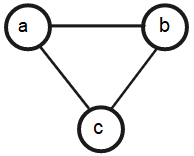
\includegraphics[width=2.3cm]{./img/trianguloabc.png} && 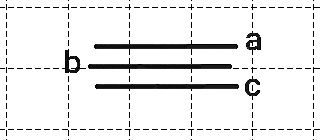
\includegraphics[width=3.5cm]{./img/b0epgTransparenciaGrade2.png} & &
    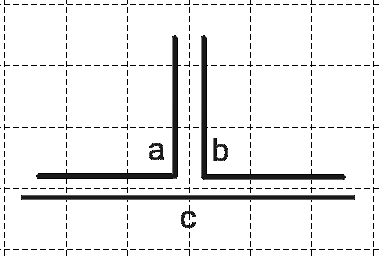
\includegraphics[width=3.5cm]{./img/b1EpgTransparenteGrade2.png}
    \\
    \footnotesize %\centering 
    (a) The  graph $C_3$ && \footnotesize(b) $B_0$-EPG representation of $C_3$ && (c) $B_1$-EPG representation of $C_3$\\
%& &  \\ \centering
%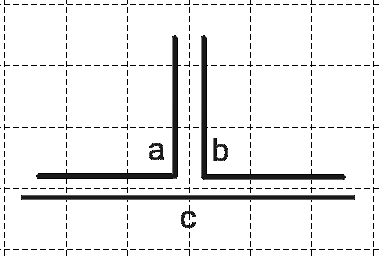
\includegraphics[width=3.5cm]{./img/b1EpgTransparenteGrade2.png} %b1epgtriangulo
 %    & 
  %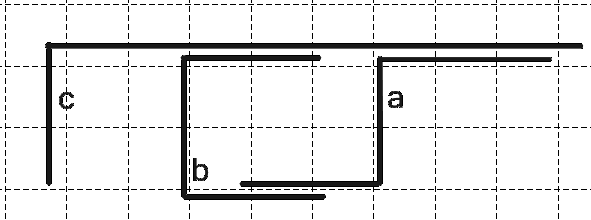
\includegraphics[width=5cm]{./img/b2epgTransparenciaGrade2.png}\\
%   \footnotesize \centering (c) $B_1$-EPG representation of $C_3$  &  \footnotesize  (d) $B_2$-EPG representation of $C_3$ \\
  \end{tabular}

 \caption{The  graph $ C_3 $  and  representations without bends and with 1 bend} \label{fig:trianguloepgRepresentacao}
\end{figure}


%A  collection $C$ of sets satisfies the Helly property when every sub-collection of $ C $ that is pairwise intersecting has at least one common element. The Helly property has this name in honor of the great Austrian mathematician Eduard Helly, who in 1923 proposed his famous theorem concerning the relation of intersecting sets.

%The study of the Helly property is useful in very diverse areas of science, and we can enumerate applications in semantics, code theory, computational biology, database, image processing, graph theory, optimization, and linear programming \cite{dourado2009}.

%Note that the representation of Figure~\ref{fig:trianguloepgRepresentacao}(b) satisfies the Helly property, while the representations of Figures~\ref{fig:trianguloepgRepresentacao}(c) and~\ref{fig:trianguloepgRepresentacao}(d) do not satisfy it.


This paper studies graphs that have an EPG-Helly representation. We prove that the problem of recognizing $ B_1$-EPG-Helly graphs is $NP$-complete.   The Helly property related to EPG representations of graphs has been studied in~\cite{golumbic2009} and \cite{golumbic2013}. In particular, they have determined the strong Helly number of $B_1$-EPG graphs. 

% recognition problem.% whose representation has the Helly property.

   %@comment retirado para o SBPO
   %Dessa forma, para situar o leitor neste contexto, são definidos na seção seguinte os principais termos utilizados ao longo deste escrito. 
 
 
 %\subsection{Basic definitions}
 Next, we describe some terminology and notation used.

%@comment falar q a diagonal não é considerada
%ver se o conceito de direção não confunde com caminho direcionado

The term \emph{grid} is used to denote the Euclidean space of integer orthogonal coordinates. Each pair of integers \emph{coordinates} are a point or vertex of the grid. The term \emph{edge of the grid}, will be used to denote a pair of vertices that are at a distance one in the grid. Two edges $e_1$ and $e_2$ are \emph{consecutive edges} when they share exactly one point of the grid. %have a common vertex. %A \emph{finite sequence of consecutive edges} is a finite sequence where every vertices are differents  
 A \emph{path in the grid} is any finite sequence of consecutive edges, without  repetition. The first and last edges of a path are called \emph{extremity edges}.
The \emph{direction of an edge} is vertical when the first coordinate of its vertices  are equal, and is horizontal when the second coordinates are equal. A \emph {bend} in a path is a pair of consecutive edges $ e_1, e_2 $ of that path, such that the directions of $ e_1$ and $ e_2$ are different. When two edges $ e_1$ and $e_2 $ form a bend, they are called \emph { bend edges}. A \emph {segment} is a set of consecutive edges with no bends. %is a path with no bends.
 Two paths are said to be \emph{edge-intersecting}, or  simply  \emph{intersecting}, if they share at least one edge. %Otherwise we say they are \emph{edge-disjoint} (or disjoint).
 Through the paper any time we say that two paths intersect, we mean they edge-intersect.  %, all intersections of paths are meant to edge intersections.

EPG graphs are the class of intersection graphs of paths in a grid~\cite{golumbic2009}. This class,  consists of the class of graphs in which its vertices are represented by paths of a grid $ Q $, such that two vertices in $ G $ are adjacent if and only if their corresponding paths intersect. If every path in a representation can be represented with at most $ k $ bends, we say that this graph $ G $ has a \emph{ $ B_k$-EPG} representation.%, and we will indicate this representation by the notation $ B_k$-EPG($ G $).
When $ k = 1 $ we say that this is a \emph{single bend} representation.


%Two sets, $ A $ and $ B $, are \emph{intersecting} $ A \cap B \neq \emptyset $. 
A family of sets is \emph{pairwise intersecting} if any two sets in the family intersect. A collection of non-empty sets $C$ satisfies the Helly property when every pairwise intersecting sub-collection $S$ of $ C $ has at least one element that is in every subset of $S$.

The Helly property can be applied to the $ B_k $-EPG representation problem, where each path is considered a set of edges. A graph $ G $ has a  $ B_k$-EPG-Helly representation if there is a $ B_k $-EPG representation of $G$ where each path has at most $ k $ bends and this representation satisfies the Helly property. %Further for all subset of pairwise intersecting paths, there is an edge common to all paths of this subset, we will indicate this representation by the notation H-$B_k$-EPG($G$). 
 Figure~\ref{fig:envelopeRepresentacoes}(a) presents two $B_1$-EPG representations of a graph with five vertices.  Figure~\ref{fig:envelopeRepresentacoes}(b)   presents 3 pairwise intersecting paths ($p(v_1), p(v_2), p(v_5)$), containing a common edge, so it is a $ B_1$-EPG-Helly representation. In Figure~\ref{fig:envelopeRepresentacoes}(c), although the three paths are pairwise intersecting, there is no common edge in all 3 paths, and therefore they do not satisfy the Helly property. 

\begin{figure}[h]
  \centering
  \begin{tabular}{ p{4cm} p{4cm} p{4cm} }
    \centering 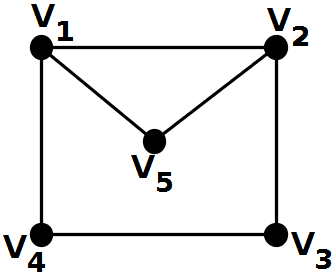
\includegraphics[width=2.5cm]{./img/envelope.png} & 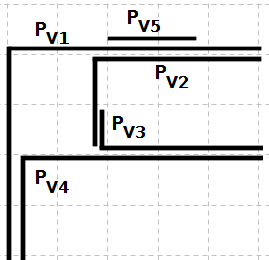
\includegraphics[width=3cm]{./img/envelopeHellyGradeTransparente.png} & 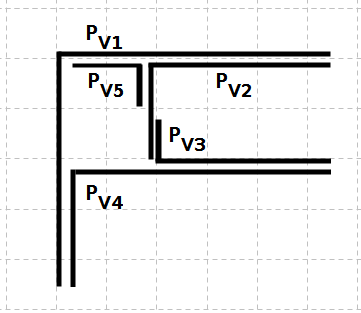
\includegraphics[width=3.4cm]{./img/envelopeNaoHellyGrade.png}
    \\
    \footnotesize \centering (a) A  graph with 5 vertices & \footnotesize(b) $B_1$-EPG representation that satisfies the Helly property & \footnotesize (c) $B_1$-EPG representation that does  not satisfy the Helly property  \\
% &&  \\ 

% \begin{tabular}[c]{@{}l@{}} 
% \hspace{3.3cm} 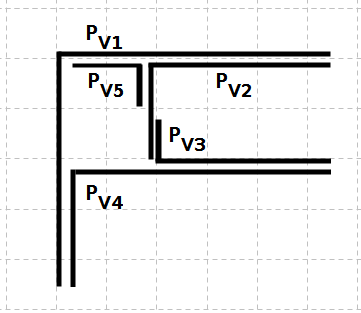
\includegraphics[width=4cm]{./img/envelopeNaoHellyGrade.png} %b1epgtriangulo
% \\
%  \hspace{3.3cm} \footnotesize (c) $B_1$-EPG representation that does\\ 
%  \hspace{3.3cm} \footnotesize not satisfy the Helly property
% \end{tabular}

% \centering &
% 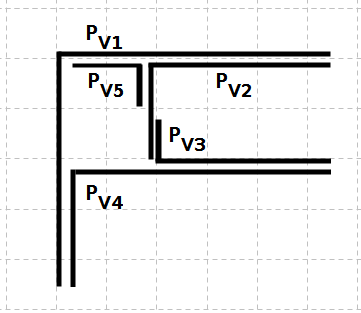
\includegraphics[width=5cm]{./img/envelopeNaoHellyGrade.png} %b1epgtriangulo
%       &
%  \\
%   \footnotesize \centering (c) $B_1$-EPG representation that not satisfies the Helly property &  &  \\
  \end{tabular}
\caption{A  graph with 5 vertices in (a) and some single bend representations: Helly in (b) and not Helly in (c)} \label{fig:envelopeRepresentacoes}
\end{figure}

%An \emph{edge (of the grid) is relevant} if at least one of its coordinates is the start, bend, or end of a path. A  \emph{maximal segment} is one whose its ends are relevant edges.  

%A $B_k$-EPG representation \emph{is normalized} when all columns $(i,i+1)$ and lines $(j,j+1)$ that have only not relevant edges in the representation have been removed. 

 %The next lemma, shows that every graph is an EPG-graph.
 
 It is easy to construct EPG representations to verify the following lemmas.
 
 \begin{lemma} \cite{golumbic2009} \label{lem:todoGrafoEpg}
 Every graph is an EPG graph.
 \end{lemma}
%  \begin{proof}
%  Let $G=(V,E)$ be a graph with vertices $v_1,\dots ,v_n$. Consider the grid $Q$ with rows $[1,\dots ,n]$ and columns $[1, 1', 2, 2', \dots, n,n']$. 
 
%  Consider the vertex $v_i$ and denote $N^+(v_i)$= $\{v_j|i<j,(i,j)\in E\}$, where $N^+(v_i)$= $\{v_{j_1}, \dots, v_{j_k}\}$ is ordered with $\{v_{j_1}< \dots < v_{j_k}\}$.   The path $P_i$ on $Q$ is defined starting horizontally from grid point $(1,i)$ to $(i,i)$, continuing vertically to $(i,j_1)$, horizontally to $(i',j_1)$, continuing vertically to $(i,j_2)$, horizontally to $(i',j_2)$, continuing vertically $(i,j_3)$, horizontally $(i',j_3)$, etc. i.e., we alternate between column $i$ and column $i'$ as we go across on each level $j_1, j_2, \dots, j_k$. %reference Figure
%  We prove that $P_i$ on the grid $Q$ is an EPG representation of $G$. For every $i<j,(v_i,v_j)\in E(G)$ if and only if the paths $P_i$, $P_j$ contain the horizontal grid edge $((i,j), (i',j))$. Moreover, no paths share vertical grid edges. Therefore the vertices in the graph are adjacent if and only if the corresponding paths share a common grid edge.
%  $\square$ \end{proof}
 
 %Moreover, the same applies to EPG-Helly graphs. 
 
 \begin{lemma}\label{lem:todoGrafoEpgHelly}
 Every graph is an EPG-Helly graph.
 \end{lemma}
%  \setcounter{proof}{1}
%   \begin{proof}
%   Let $G$ be a graph with $n$ vertices $v_1, v_2, \dots, v_n$ and $\mu$ maximal cliques $C_1, C_2, \dots , C_{\mu }$. We construct an EPG-Helly representation of $G$, using a grid $Q$ of size $(\mu \times 2n)$. The lines correspond to the maximal cliques and are numbered $1, 2, \dots , \mu$. Each vertex $v_j$ corresponds to the pair of columns $j, j+n$. Each maximal clique $C_i$ is mapped into an edge $(i,n), (i,n+1)$. Each path $P_j$ contains all edges $(i,n), (i,n+1)$ corresponding to the maximal cliques $C_i$ containing $v_i$.
  
%   Moreover, two distinct paths $P_j,P_k$ intersect at the edges corresponding to the maximal cliques containing $v_j,v_k$.
  
%   Let $v_j \in V(G)$, consider the maximal cliques containing $v_j$ in ascending order of their indices. The path $P_j$ representing $v_j$, start at vertex $(1,j)$ of $Q$ and descends column $j$ until $(i,j)$, where $C_i$ is the first clique containing $v_j$ then $P_j$ bends at vertex $(i,j)$ and proceeds to the right, travesses edge $(i,n), (i,n+1)$ representing $C_i$. Then $P_j$ proceeds further on line $i$ until reaching vertex $(i, j+n)$, where it bends again, descending column $j+n$ until reaching vertex $(l,j), l>i$, where $C_l$ is the next maximal clique containing $v_j$ where it bends again. It proceeds in line $l$, travessing edge $(l,n),(l,n+1)$, and so on, until all edges of $Q$ corresponding to the maximal cliques containing $v_j$ have been travessed by $P_j$.   
  
% It follows that two distinct paths, $P_j$ and $P_q$, intersect exactly at the lines corresponding to the maximal cliques containing both $v_j$ and $v_q$.  
%   $\square$ \end{proof}
 
%  Figure~\ref{fig:gradeDemonstracao} shows the grid $Q$ and the path $P_2$ corresponding to the vertex $v_2 \in V(G)$, contained in maximal cliques $C_2, C_4$ and $C_5$ of $G$.
 
%   \begin{figure}[htb]	
\center%6.3
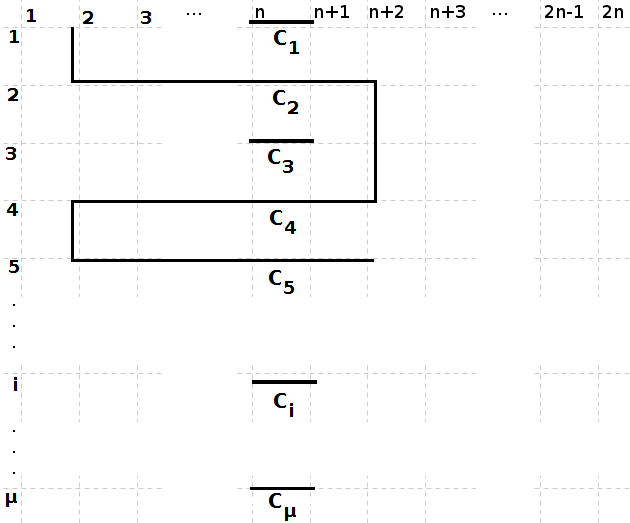
\includegraphics[width=8cm]{./img/grade3.png}
%clausulaGadgetGFCompletaSBPO
\caption{Representation of the path $P_2$ corresponding to vertex $v_2$ contained in cliques $C_2, C_4$ and $C_5$}
\label{fig:gradeDemonstracao}
\end{figure}
 
 
 \begin{corollary}\label{cor:maxCliques}
 Every graph $G$ containing $\mu$ maximal cliques admits a $B_{2\mu -1}$-EPG-Helly representation. %in a grid $Q$ of dimension $(\mu \times 2n)$.
 \end{corollary}
 
Most of the proofs of the paper are detailed in the Appendix.
 
\section{Basic EPG representations}
%{The Classes $B_1$-EPG and $B_1$-EPG-Helly}

% Although classes $B_1$-EPG and $ B_1$-EPG-Helly do not coincide, see Lemma~\ref{lem:octaedronaohelly}, the same does not occur for classes $ B_0$-EPG and $ B_0$-EPG-Helly, as observed in Lemma~\ref{lem:b0epg}.

% \begin {lemma} \label{lem:b0epg}
% Every $ B_0$-EPG representation satisfies the Helly property.
% \end {lemma}
% \begin {proof}
% Assume by contradiction that there exists a graph $G$ that admits a $ B_0$-EPG representation that does not satisfy the Helly property. Then, this representation has a minimal collection $ P = \{p (v_1), p (v_2), \ldots, p (v_k) \} $ of mutually intersecting paths such that $$ p(v_1) \cap p(v_2 ) \cap \cdots \cap p(v_k) = \emptyset, k \geq 3. $$
% By minimality, we know that $ \bar{P_1} = P \setminus \{p (v_1) \}$, $ \bar {P_2} = P \setminus \{p(v_2) \} $ and $ \bar {P_3 } = P \setminus \{p (v_3) \} $ are mutually intersecting and satisfy the Helly property.
% Thus, there are the following distinct segments $ s_{\bar{P_1}}, s_{\bar {P_2}}, s_{\bar {P_3}}$ associated with the intersection of the paths in $ \bar {P_1},  \bar {P_2} $ and $ \bar {P_3} $. Since the representation has no paths with bends, then we know that the paths in $ P$ are on the same line.
% Without loss of generality, we can assume that $ s_{ \bar {P_1}}, s_{ \bar {P_2}}$ and $ s_{ \bar {P_3}}$ occur from left to right in this order.
% Since $ s_{\bar {P_3}}$ and $ s_{\bar {P_1}}$ intersect $ p(v_2) $, and $ p (v_2) $ is in path without bend, then $ p (v_2) $ intersects $ s_{\bar {P_2}}$. Then we have a contradiction, since $ s_{\bar {P_2}} $ intersects all paths in $ P $, contradicting the hypothesis of $ p(v_1) \cap p(v_2) \cap \cdots \cap p(v_k) = \emptyset $.
% \end {proof}
% %%%%%%%%%

% \begin{coro}
% The  $B_0$-EPG class coincides with the $B_0$-EPG-Helly class.
% \end{coro}

% $B_0$-EPG graphs coincide with the interval graphs class. The problem of interval graph recognition can be solved in linear time~\cite{booth1976}. Although the problem of $ B_1$-EPG graph recognition is NP-complete \cite {heldt2014}, the $ B_1$-EPG-Helly graphs form a subclass properly contained in $ B_1$-EPG. See Figure~\ref{fig:diagramaEPG}, and the complexity of its recognition was in open. 

% Lemma \ref{lem:octaedronaohelly} shows that the classes $ B_1$-EPG and $ B_1$-EPG-Helly are distinct, observing the graph octahedron $ O_3 $, see Figure~\ref{fig:octaedro}(a), which presents a minimal $B_1$-EPG representation, without considering isomorphisms, as in Figure~\ref{fig:octaedro}(b) for its representation. The octahedron graph $ O_3 $ belongs to $ B_1$-EPG but does not belong to $ B_1$-EPG-Helly.

% \begin{figure}[htb]	
\center%6.3
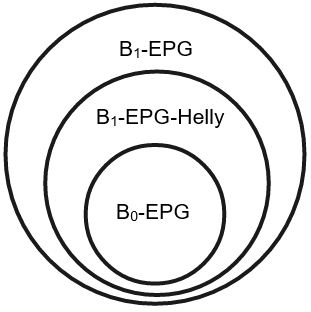
\includegraphics[width=3.5cm]{./img/diagramaClassesEPG.png}
\caption{Hierarchical diagram of some EPG classes}
\label{fig:diagramaEPG}
\end{figure}

In this section we examine the $B_1$-EPG representations of a few interesting graphs. First, we consider EPG representations of $C_4$'s.

%By the results of \cite{golumbic2009}, in Lemma ~\ref{lem:representacaoC4}, every induced cycle of size 4 in a $ B_1$-EPG  representation  of $C_4$ has only a few possible representations.

\begin{definition} \label{defi:tortasFrame}

Let $ Q $ be a grid and let $ (a_1, b),$ $(a_2, b),$ $(a_3, b),$ $(a_4, b)$ be a 4-star as depicted in Figure~\ref{fig:piesInGrid}(a). Let $ \mathcal{P} = \{P_1, \dots , P_4\}$ be a collection of paths each containing exactly two edges of the $4$-star:

\begin{itemize}
\item A \emph{true pie} is a representation where each $P_i$ of $ \mathcal{P} $ forms a bend in $b$.

\item A \emph {false pie} is a representation where two of the paths $P_i$ do not contain bends, while the remaining two do not share an edge. 

%In false pie only 2 paths not adjacent do bend in $b$.

\begin{figure}[htb]
  \centering
%segundo bloco de figuras
  \begin{tabular}{c c c c c }
    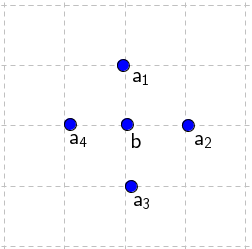
\includegraphics[width=3.5cm]{./img/disposicaoTortaGrid.png}    
    & &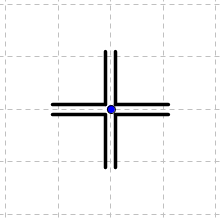
\includegraphics[width=3.5cm]{./img/truePieGrid.png} 
    & &
 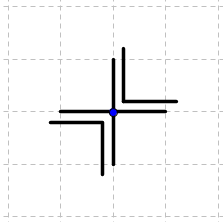
\includegraphics[width=3.5cm]{./img/falsePieGrid.png} \\%[\abovecaptionskip]
    {\footnotesize (a) 4-star in grid}  & &  {\footnotesize (b) True pie} & & {\footnotesize (c) False pie} %\label{fig:frame}
  \end{tabular}
  \caption{$B_{1}$-EPG representation of the induced cycle of size 4 as pies with emphasis in center $b$}\label{fig:piesInGrid}
\end{figure} 

\end{itemize}
\end{definition}
%In both cases the point $b$ is called \emph{center}, see Figures~\ref{fig:piesInGrid}(b) and~\ref{fig:piesInGrid}(c). There are edge-intersections $ (a_1, b), (a_2, b), (a_3, b), (a_4, b)$ called \emph{central rays}, see Figure~\ref{fig:piesInGrid}.

\begin{definition} \label{defi:tortasFrame2}
 Consider a rectangle of any size with 4 corners at vertices $ (x_1, y_1);$ $(x_2, y_1);$ $(x_2, y_2);$ $(x_1, y_2) $, positioned as in  Figure~\ref{fig:frameInGrid}. A \emph{frame} is a representation containing 4 paths $\mathcal{P} =  \{ P_1, \dots, P_4\} $, each having a bend in a different corner of a rectangle, and such that the  sub-paths $ P_1 \cap P_2, P_2 \cap P_3, P_3 \cap P_4, P_4 \cap P_1 $, share at least one edge. While the sub-paths $ P_2 \cap P_4 $ and $ P_1 \cap P_3 $ do not share edges.

\begin{figure}[htb]
  \centering
%segundo bloco de figuras
  \begin{tabular}{c c c c c }
    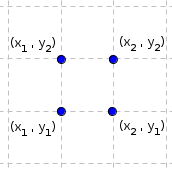
\includegraphics[width=3.5cm]{./img/dispositionFrameInGrid.png}    
    %& &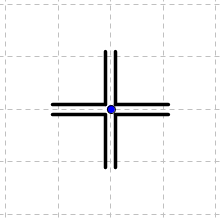
\includegraphics[width=4cm]{./img/truePieGrid.png} 
    & &
 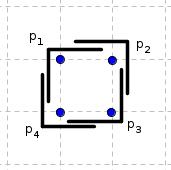
\includegraphics[width=3.5cm]{./img/frameInGrid.png} \\%[\abovecaptionskip]
    {\footnotesize (a) Points of the coordinates of bends of a frame}  
    %& &  {\footnotesize (b) True pie} 
    & & {\footnotesize (c) Paths of a frame} %\label{fig:frame}
  \end{tabular}
  \caption{$B_{1}$-EPG representation of the induced cycle of size 4 as frame}\label{fig:frameInGrid}
\end{figure} 

\end{definition}


%% \begin{figure}[htb]	
% \center%6.3
% 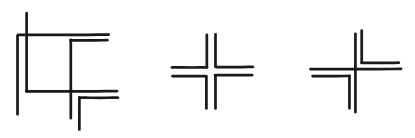
\includegraphics[width=10cm]{./img/representacaociclotam4.png}
% \caption{$B_{1}$-EPG representation of the induced cicle of size 4: frame (in left), true pie (center) and false pie (in right), \cite{golumbic2009}.}

% \end{figure}

\begin{figure}[htb]
  \centering
%segundo bloco de figuras
  \begin{tabular}{c c c c c }
    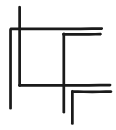
\includegraphics[width=2.3cm]{./img/representacaociclotam41.png}  
    & &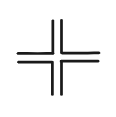
\includegraphics[width=2.5cm]{./img/representacaociclotam42.png} 
    & &
 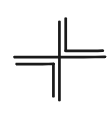
\includegraphics[width=2.5cm]{./img/representacaociclotam43.png} \\%[\abovecaptionskip]
    {\footnotesize (a) Frame}  & &  {\footnotesize (b) True pie} & & {\footnotesize (c) False pie} %\label{fig:frame}
  \end{tabular}
  \caption{$B_{1}$-EPG representation of the induced cycle of size 4}\label{fig:ciclotam4}
\end{figure} 


\begin{lemma}\label{lem:representacaoC4}
\cite{golumbic2009} Every  $C_4$ that is an induced subgraph of a graph $ G $ corresponds, in any representation, to a true pie, a false pie, or a frame.
\end{lemma}
% \begin{proof} Consider a collection of paths $ P = \ {P_1, \dots, P_4}$ of a grid $ Q $ in a $ B_1$-EPG representation of the graph $G$.

% Consider $ C_4 = (v_1, v_2, v_3, v_4) $ that is a chordless 4-cycle in $ G$. Consider $P_i$ the path in $ G $ that corresponds to $v_i $.
% Suppose $ \displaystyle \bigcap _{P_i \in P} P_i \neq \emptyset $, then clearly $ \displaystyle \bigcap _{P_i \in P} P_i = {b} $, for some point $ b $ of the grid. Since each vertex in $ C_4 $ has exactly 2 neighbors, each path $ P_i $ contains exactly two edges of the grid with end point $ b$. Thus, we obtain a star subgraph with center point $ b $ and edges $ (a_1, b), (a_2, b), (a_3, b), (a_4, b)$.
% Without loss of generality, $ P_1 $ contains the edges $ (a_1, b), (a_2, b) $ of the grid. If $ P_2 $ contains $ (a_2, b), (a_3, b) $ or $ (a_1, b), (a_4, b) $, then we get a true pie. Otherwise, $ P_2 $ contains the edges $ (a_2, b), (a_4, b) $ or $ (a_1, b), (a_3, b) $ and we obtain a false pie.

% Otherwise, $ \displaystyle \bigcaP_ {P_i \in P} P_i = \emptyset$. Suppose $ P_1 $ is a path without bend. Each of the $ P_2 $ and $ P_4 $ paths share an edge with $ P_1 $ but do not share a common edge with any other path. If $ P_2 $ and $ P_4 $ do not have a bend, then we get a interval representation of $ C_4 - v_3 $. However, it is not possible to add a $ P_3 $ path with at most of one bend. Similarly, if $ P_2 $ and $ P_4 $ have a single bend, the $ P_3 $ path can not be added either. Therefore, $ P_1 $ has a single bend.

% By symmetry, we assume that all $ P_i $ must has a single bend. Moreover, two paths can not have a bend on a common point in the grid. Thus, we obtain a rectangular subgraph with angles $ (x_1, y_1), (x_2, y_1), (x_2, y_2), (x_1, y_2) $, where $ P_1 $ bends at $ (x_1, y_1) $, $ P_2 $ bends at $ (x_2, y_1) $, $ P_3 $ bends at $ (x_2, y_2) $, and $ P_4 $ bends at $ (x_1, y_2) $, forming a frame.
% $\square$ \end{proof}

\begin{definition}
%A edge is \emph{unnecessary} if its removal keeps the intersections and not intersection of the representation. 
A $B_k$-EPG representation is \emph{minimal} 
when its set of edges  does not properly contain another $B_k$-EPG representation. 
%when all unnecessary edges are removed.
\end{definition}

The \textit{octahedral} graph is the graph containing 6 vertices and 12 edges, depicted  in Figure~\ref{fig:octaedro}(a). Next, we consider representations of the octahedral.

\begin{lemma}\label{lem:octaedronaohelly}
The octahedral graph $O_3$ has a unique minimal  $ B_1$-EPG representation.%, without considering isomorphisms.
\end{lemma}
% \begin{proof}
% The octahedral graph $ O_3 $ has in its constitution induced cycles of size 4 ($ C_4$'s). 
% Take an induced $ C_4 $ subgraph  of the octahedral $ O_3 $. The pairs of non-adjacent vertices of the induced $C_4$ are false twins whose neighborhoods are the remaining of vertices of the induced $C_4$. Each of the vertices outside the $C_4$ are adjacent to all vertices of the $C_4$. Thus, if in a $ B_1$-EPG representation of $C_4$, the $ C_4 $ is represented as a frame, no single bend path can simultaneously intersect the 4 paths representing the vertices of the induced $ C_4 $. Therefore, we conclude that the frame structure can not be part of a $ O_3 $ representation.

% With the same reasoning, take a $ B_1$-EPG representation of $C_4$ where the induced $ C_4 $ subgraph is represented as true pie or false pie. When adding the false twin vertices, which are neighbors of all vertices of $ C_4 $ taken from $ O_3 $, both representations converge to the structure represented in Figure~\ref{fig:octaedro}(b). 
% $\square$ \end{proof}

 \begin{figure}[h]
  \centering
  
%segundo bloco de figuras
  \begin{tabular}{@{}c@{} p{1.5cm} @{}c@{} }
   \centering 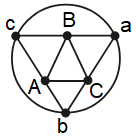
\includegraphics[width=2.5cm]{./img/octaedro.png} & &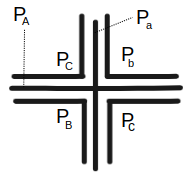
\includegraphics[width=2.9cm]{./img/representacaoOctaedro.png}  \\[\abovecaptionskip]
    \footnotesize \centering (a) The octahedral $O_3$ graph  & &  \footnotesize(b) $B_1$-EPG representation of the graph $O_3$
  \end{tabular}

 \caption{The octahedral $O_3$ graph and its  $B_1$-EPG representation}\label{fig:octaedro}
\end{figure}\vspace{-.5cm}

By Lemma ~\ref{lem:octaedronaohelly},  $ O_3 $ has a unique minimal $B_1$-EPG representation, up to isomorphisms, as depicted in Figure~\ref{fig:octaedro}(b). The paths $ p(a), p(b) $ and $ p(c) $  do not satisfy the Helly property. Therefore $O_3 \notin B_1$-EPG-Helly. 

\section{Membership in $\mathcal{NP}$} 

{\sc $B_k$-EPG-Helly recognition} problem can be formally described as follows:
\begin{table}[h!]
\centering
%\caption{My caption}
%\label{my-label}
\begin{tabular}{ll}
\hline \hline
\multicolumn{2}{c}{\sc $B_k$-EPG-Helly Recognition}                         \\ \hline \hline 
\emph{Input}: & A graph $G$, and an integer $k$.\\
%~ & ~ \\
\emph{Goal:}  & \begin{tabular}[c]{@{}p{9.5cm}}
Determine if there is a set of $k$-bend paths \\ $\mathcal{P} = \{P_1, P_2, \ldots, P_n\} $ in a grid $ Q $ 
such that:\\ 
$\bullet$ \ \ \ $u,v\in V(G)$ are adjacent in $G$ if only if $P_u,P_v$\\ \hspace{0.6cm} share an edge in $Q$; and\\
$\bullet$ \ \ \ $\mathcal{P}$ satisfies the Helly property.
\end{tabular} \\ \hline
\end{tabular}
\end{table}


%Let $(G,k)$ be an instance of {\sc $B_k$-EPG-Helly recognition}, and
%let $\mu$ be the number of maximal cliques of $G$. By Corollary~\ref{cor:maxCliques}, $G$ admits a $B_{2\mu -1}$-EPG-Helly representation. Therefore, since $\mu \leq 2^{|V(G)|}$, it follows that if $k\geq 2^{|V(G)|+1}-1$ then $G$ is a trivial $yes$-instance of {\sc $B_k$-EPG-Helly recognition}. Thus, without loss of generality, we can assume that $k< 2^{n+1}-1$. 

%In this paper we are interested in characterizing the complexity of the $B_1$-EPG-Helly recognition problem, whose formal definition is presented next:
In this section, we show that the problem $B_k$-EPG-Helly recognition, where $k$ is bounded by a polynomial in $|V(G)|$, belongs to $\mathcal{NP}$. 


A (positive) certificate for the {\sc $B_k$-EPG-Helly recognition} problem consists of a grid $Q$, a set $\mathcal{P}$ of $k$-bend paths of $Q$, which have a one-to-one correspondence with the vertex set $V(G)$ of $G$, such that, for each pair of distinct paths $P_i, P_j\in \mathcal{P}, P_i\cap P_j \neq \emptyset $ if and only if the corresponding vertices are adjacent in $G$. Furthermore, $\mathcal{P}$ satisfies the Helly property.


%The following concepts are central to our purposes. A \emph{relevant edge} in a  $B_k$-EPG representation is one which is either an extremity edge or a bend edge. Therefore each path with at the most $k$ bends can have $2(k+1)$ relevant edges, and any $B_k$-EPG representation contains at most $2|\mathcal{P}|(k+1)$ relevant edges.

%The input for the verification algorithm of the certificate is a $B_k$-EPG representation $R$ containing a collection $\mathcal{P}$ of paths, $|\mathcal{P}|=|V(G)|$, where each path $P_i \in \mathcal{P}$ is given by its set of relevant edges plus the set of relevant edges of the paths that intersect $P_i$, the relevant edges are given in the order that they appear in the path. This coding format for the paths allow us to verify if each set of relevant edges really represents a path and the paths intersections correspond to the edges of the graph in polynomial time.

The following are key concepts that make it easier to control the size of an EPG representation. A relevant edge of a path in a $B_k$-EPG representation is one which is either an extremity edge or a bend edge of the path. Therefore each path with at the most $k$ bends can have up to $2(k + 1)$ relevant edges. Any $B_k$-EPG representation contains at most $2|\mathcal{P}|(k + 1)$ distinct relevant edges. 

The certificate for a verification algorithm  that shows that a graph is a $B_k$-EPG Helly graph is a  $B_k$-EPG representation $R$ containing a collection $\mathcal{P}$ of paths, $|\mathcal{P}| = |V(G)|$, such that  each path $P_i \in P$ is given by its set of relevant edges along with the relevant edges of each path that intersects $P_i$.  The relevant edges for each path are given in the order that they appear in the path, so as to make checking that the edges correspond to a unique path with at most $k$ bends straightforward.  This representation is also handy for checking that the paths form an intersection model for $G$.

In order to verify in polynomial time that the input is in fact is a certificate for the problem, we have to assert the following:

\begin{enumerate}[label=(\roman*)]
\item The sequence of relevant edges of a path $P_i\in \mathcal{P}$ determines $P_i$ in polynomial time; \label{it:bullet1}

\item Two paths $P_i, P_j \in \mathcal{P}$ intersect if and only if they intersect in some relevant edge; \label{it:bullet2}

\item The set $\mathcal{P}$ of relevant edges satisfies the Helly property.  \label{it:bullet3}
\end{enumerate}


%The following lemma shows condition~\ref{it:bullet1} holds.

The following lemma states that condition~\ref{it:bullet1} holds. 



\begin{lemma}\label{lem:verify1}
%Each path $P_i$ can be determined in polynomial time, from the considered sequence of edges.
Each path $P_i$ can be determined uniquely in polynomial time by the sequence of its relevant edges.
\end{lemma}

% \begin{proof}
% It is easy to verify that~\ref{it:bullet1} is true, consider the sequence of relevant edges of some path $P_i\in \mathcal{P}$. Start from an extremity edge of $P_i$. Let $t$ be the line (column) containing the last considered relevant edge. The next relevant edge $e'$ in the sequence, must be also contained in line (column) $t$. If $e'$ is an extremity edge, the process is finished and the path has been determined. It contains all edges between the considered relevant edges in the sequence. Otherwise, if $e'$ is a bend edge , the next relevant edge is the second bend edge $e''$ of this same bend, which is contained in some column (line) $t'$. The process continues until the second extremity edge of $P_i$ is located.   

% With the above procedure, we can determine in $O(k+|V(G)|)$ time, whether path $P_i$ contains any given edge of the grid $Q$. Therefore, the sequence of relevant edges of $P_i$ uniquely determines $P_i$.
% $\square$ \end{proof}

%The lemma below shows that~\ref{it:bullet2} holds.
Next we assert property~\ref{it:bullet2}.

\begin{lemma}\label{lem:relevantEdges}
%Let $R$ be a $B_k$-EPG representation of $G$, and $P_1, P_2 \in \mathcal{P}$ paths of $R$. Then $P_1, P_2$ are intersecting paths if and only if they contain a common relevant edge.
Let $\mathcal{P}$ be the paths in a $B_k$-EPG representation of $G$, and let $P_1, P_2\in \mathcal{P}$. Then $P_1$, $P_2$ are intersecting paths if and only if their intersection contains at least one relevant edge.
\end{lemma}

% \begin{proof}
% If $P_1, P_2$ contain a common relevant edge there is nothing to prove. Otherwise, assume that $P_1, P_2$ are intersecting and we show they contain a common relevant edge. Without loss of generality, suppose $P_1, P_2$ intersect at line \textit{i} of the grid, in the  $B_k$-EPG representation $R$. The following are the possible cases that may occur:

% \begin{itemize}
% \item \textbf{Case 1:} Neither $P_1$ nor $P_2$ contain bends in line \textit{i}. 

% Then $P_1$ and $ P_2$  are entirely contained in line \textit{i}. Since they intersect, either $P_1, P_2$  overlap, or one of the paths contains the other. In any these situations, they intersect in a common extremity edge, that is a relevant edge.

% \item \textbf{Case 2:} $P_1$ does not contain bends in \textit{i}, but $ P_2$ does contain.

% If some bend edge of $P_2$ also belongs to $P_1$, then $P_1, P_2$  intersect in  a relevant edge. Otherwise, since $P_1, P_2$  intersect, the only possibility is that the intersection contains an extremity edge of $P_1$ or $ P_2$. Hence the paths intersect in relevant edge.  

% \item \textbf{Case 3:} Both $P_1$,  $P_2$ contain bends in \textit{i}

% Again, if the intersection occurs in some bend edge of $P_1$  or $P_2$, the lemma follows. Otherwise, the same situation as above must occur, that is $P_1, P_2$  must intersect in same extremity edge.
 
% \end{itemize}
% In any of the cases, $P_1$ and $P_2$ intersect in some relevant edge.
% $\square$ \end{proof}

The two previous lemmas let us check that a certificate is an actual $B_k$-EPG representation of a given graph $G$.  The next lemma says we can actually verify in polynomial time that the representation encoded in the certificate is a Helly representation. Fortunately we do not need to check every subset of intersecting paths  of the representation to make sure they have a common intersection. 

% \begin{enumerate}[label=\roman*]
% \setcounter{enumi}{2}
% \item The set $\mathcal{P}$ of relevant edges satisfies the Helly property. The following lemma shows the above condition.
% \end{enumerate}

\begin{lemma}\label{lem:verify3}
%Let $\mathcal{P}$ be the set of relevant edges of a $B_k$-EPG representation $R$ of a graph $G$. We can verify that $R$ is Helly representation in polynomial time.
Let $\mathcal{P}$ be a collection of paths encoded as a sequence of relevant edges that constitute a  $B_k$-EPG representation of a graph $G$. We can verify in polynomial time if $\mathcal{P}$ has the Helly property.
\end{lemma}
%\setcounter{proof}{2}

\begin{proof}
%Let $\mathcal{T}$ be the set of relevant edges of $R$. We consider each triple $T_i$ of edges of $\mathcal{T}$. Let $\mathcal{P}_i$ be the set of paths of $R$ containing at least two the relevant edges of $T_i$. By Gilmore's theorem~\cite{bergeDuchet1975} the paths of $\mathcal{P}_i$  contain a common edge if only if  $R$ is a Helly representation.  By Lemma~\ref{lem:relevantEdges} they contain a common relevant edge. Since there is a polynomial number of relevant edges, we can identify such a common edge, in polynomial time, and confirm that $R$ is in fact Helly. Since the number of triples is also polynomial, the lemma follows.
Let $T$ be the set of relevant edges of $\mathcal{P}$. Consider each triple $T_i$ of edges of $T$ . Let $P_i$ be the set of paths of $\mathcal{P}$ containing at least two of the edges in the triple  $T_i$. By Gilmore’s theorem \cite{bergeDuchet1975} $\mathcal{P}$ has the Helly property if an only if the subset of paths $P_i$  corresponding to each triple  $T_i$  has a non-empty intersection.  By Lemma~\ref{lem:relevantEdges} it suffices to examine the intersections on relevant edges. Therefore a polynomial algorithm for checking if $\mathcal{P}$ has the Helly property could examine each of the subsets $P_i$, and for each relevant edge $e$ of a path in $P_i$, to compute the number of paths in $P_i$ that contain $e$. $\mathcal{P}$ has the Helly property if and only if for every  $P_i$  there exists some relevant edge that is present in all paths in $P_i$,  yielding a non-empty intersection.
$\square$ \end{proof}


\begin{coro}\label{cor:comumAtodos}
Let ${\mathcal P}$ be a set a pairwise intersecting paths in a $B_k$-Helly representation of a graph $G$. Then the intersection of all paths of  ${\mathcal P}$ contains at least one relevant edge.
\end{coro}

Note that the property described in Corollary~\ref{cor:comumAtodos} is due to Gilmore's Theorem~\cite{bergeDuchet1975}, and it applies only to representations that satisfy Helly's property.

\medskip

%The next theorem follows immediately from (i), (ii) and (iii).

%\begin{theorem} \label{teo:nppertinencia}
%A $B_k$-EPG representation of $G$ can be verified in polynomial time, for $k = \mathcal{O}(|V (G)|^c)$ for any constant  $c$.
%A $B_k$-EPG representation of $G$ can be verified in polynomial time, for $k\leq |V(G)|^c$, for some fixed integer c.
%\end{theorem}


\begin{lemma}\label{lem:gridPolinomial}
Let $G$ be a $B_k$-EPG-Helly graph. Then $G$ admits a $B_k$-EPG-Helly representation on a grid of size at most $4n(k+1) \times 4n(k+1)$.
\end{lemma}
\begin{proof}
Let $R$ be a $B_k$-EPG representation of a graph $G$ on a grid $Q$ with the smallest possible size.
Let $\mathcal{P}$ be the set of paths of $R$. Note that $|\mathcal{P}|=n$.
A counting argument shows that there are at most $2|\mathcal{P}|(k+1)$ relevant edges in $R$. 
 If $Q$ has a pair of consecutive columns $c_i,c_{i+1}$ neither of which contains relevant edges of $R$, and such that there is no relevant edge crossing from $c_i$ to $c_{i+1}$, then we can contract each edge crossing from $c_i$ to $c_{i+1}$ into single vertices so as to obtain a new  $B_k$-EPG representation of $G$ on a smaller grid, which is a contradiction. An analagous argument can be applied to pairs of consecutive lines of the grid.
 Therefore the grid $Q$ is such that each pair of consecutive columns and of consecutive lines of $Q$  has at least one relevant edge of $R$ or contains a relevant edge crossing it.  
  Since $Q$ is the smallest possible grid for representing $G$ then the first line and the first column of $Q$ must both contain at least one point belonging to some relevant edge of $R$. 
Thus, if $G$ is $B_k$-EPG then it admits a $B_k$-EPG representation on a grid of size at most $4|\mathcal{P}|(k+1) \times 4|\mathcal{P}|(k+1)$.
In addition, if $R$ is a $B_k$-EPG-Helly representation then, by Corollary~\ref{cor:comumAtodos},  $R'$ is also a  $B_k$-EPG-Helly representation.
\qed
\end{proof}

\begin{theorem}\label{teo:nppertinencia}
{\sc $B_k$-EPG-Helly recognition} is in $\mathcal{NP}$, whenever $k$ is bounded by a polynomial function of $|V(G)|$.
\end{theorem}
\begin{proof}
By Lemma~\ref{lem:gridPolinomial} and the fact that $k$ is bounded by a polynomial function of $|V(G)|$, it follows that the collection $\mathcal{P}$ can be encoded through its relevant edges with $n^{\mathcal{O}(1)}$ bits.

Finally, by Lemmata~\ref{lem:verify1}, \ref{lem:relevantEdges} and \ref{lem:verify3}, it follows that one can verify in polynomial-time on the size of $G$ whether $\mathcal{P}$ is a family of paths encoded as a sequence of relevant edges that constitute a $B_k$-EPG-Helly representation of a graph $G$.
\qed
\end{proof}

\section{$NP$-hardness}\label{sec:sectionDispositivoClausula}

Now we will prove that  $B_1$-EPG-Helly graph recognition is $NP$-complete. For this prove we set up a reduction from {\sc Positive (1 in 3)-3SAT} defined  as follows:

\begin{table}[h!]
\centering
%\caption{My caption}
%\label{my-label}
\begin{tabular}{ll}
\hline \hline
\multicolumn{2}{c}{\sc Positive (1 in 3)-3SAT}                                \\ \hline \hline 
\emph{Input}: & \begin{tabular}[c]{@{}l@{}} A set $X$ of positive variables; a collection $\mathcal{C}=\{C_1,C_2,\ldots,C_m\}$ of clauses on $X$\\ such that for each $C_i\in \mathcal{C}$, $|C_i|= 3$.
\end{tabular} \\
~ & ~ \\
\emph{Goal:}  & \begin{tabular}[c]{@{}l@{}} 
Determine if there is an assignment of values to the variables \\in $ X $ so that every clause in $\mathcal{C}$ has exactly one true literal.
\end{tabular} \\ \hline
\end{tabular}
\end{table}

{\sc Positive (1 in 3)-3SAT } is a well known $NP$-complete problem (see \cite{johnson1979}, problem [L04], page 259). {\sc Positive (1 in 3)-3SAT} remains $NP$-complete when the incidence graph of the input CNF (Conjunctive Normal Form) formula is a planar graph~\cite{mulzer2008minimum}.

Given a formula $F$ that is an instance of {\sc Positive (1 in 3)-3SAT} we will present a polynomial-time construction of a graph $ G_F$ such that $ G_F $ is $ B_1$-EPG-Helly if and only if $ F $ is satisfiable. This graph will contain an induced subgraph $ G_c$ with 12 vertices (called \emph {clause gadget}) for every clause $ c \in C $, and an induced subgraph (\emph {variable gadget}) for each variable $ x_j$, containing a special vertex  $ v_j$, plus a \emph{base gadget}  with 55 additional vertices.

%Since a Sun graph $S_4$ whose center is a cycle of size 4 and adding a false twin to each vertex of $S_4$ that is not a member of central induced cycle then we have the graph $H$. 
We will use a graph $H$ isomorphic to the graph presented in Figure~\ref{fig:gadgetBase}, as a gadget to perform the proof. For each clause $c$ of $F$ of the target problem, we will have a \emph{clause gadget} isomorphic to $H$, denoted by $G_c$. %The graph $H$ consists of subgraphs whose $B_1$-EPG representations are well known, such as: cycles of sizes 3 and 4.

\begin{figure}[htb]	
\center%6.3
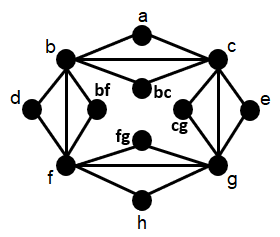
\includegraphics[width=4.5cm]{./img/gadgetBase.png}
\caption{The partial gadget graph $H$}
\label{fig:gadgetBase}
\end{figure} 

%\subsection{Definition}\label{sec:reducao}%The problem reduction}

The reduction of a formula $F$ from  {\sc Positive (1 in 3)-3SAT}  to a particular graph $G_F$ such that $G_F$ has a $B_{1}$-EPG-Helly representation if only if $F$ is satisfiable, it is given below.

\begin{definition}\label{sec:reducao}
Let $F$ be a CNF-formula with no negative literals, in which every clause has exactly three literals. The graph $G_F$ is constructed as follows:

\begin{enumerate}
\item For each clause $C_i \in F$ create a  \textit{clause gadget} $G_{c}$, isomorphic to  graph $H$;

\item For each variable $x_{j}$ create a \emph{variable vertex} $v_{j}$ that is adjacent to the vertex $a$, $e,$ or $h$ of $G_c$, when $x_{j}$ is the first, second or third variable in $C_i$, respectively;

\item For each variable vertex $v_{j}$, construct a \emph{variable gadget} formed by adding two copies of $H$, $H_1$ and $H_2$, and making $v_j$ adjacent to the vertices of the 2 triangles $(a, b, c)$ in  $H_1$ and $H_2$.

 %where $v_{j}$ is  adjacent to all vertices of the triangle (a,b,c);%; (c,e,g); (g,f,h); or (b,d,f)) of each $H_1$ and $H_2$; 

%\item The  subgraph induced by \emph{variable vertex}  $v_{j}$, and also $V(H_1)$ and $V(H_2)$ will be called \emph{variable gadget}; 

\item Create a vertex $V$, that will be used as vertical reference of the construction, and add edges from $V$ to each vertex  $d$;%$d \in V(G_c)$;

\item Create a bipartite graph $K_{2,4}$ with a particular vertex $T$ that is in the largest stable set. This vertex is nominated \emph{true vertex}. $T$ is adjacent to all $v_{j}$ and also to $V$;

\item Create two  graphs isomorphic to $H$, $G_{B1}$ and $G_{B2}$. The vertex $T$ is connected to each vertex vertices of the triangle (a,b,c) in $G_{B1}$ and $G_{B2}$;


\item Create two graphs isomorphic  to $H$, $G_{B3}$ and $G_{B4}$. The vertex $V$ is connected to each vertex of the triangle (a,b,c) in $G_{B3}$ and $G_{B4}$;

\item The  subgraph induced by vertices $V(K_{2,4})$, $T$ and $V$,  $V(G_{B1})$ and $V(G_{B2})$, and also $V(G_{B3})$ and $V(G_{B4})$ will be referred to as the  \emph{base gadget}. 
\end{enumerate}
\end{definition}


Figure~\ref{fig:exemploGrafoGF} illustrates how this construction works on a small formula. %represents the graph that would be obtained when the previous construction is applied to the formula $ F = (x_1 + x_2 + x_3) \wedge (x_2 + x_3 + x_4) \wedge (x_3 + x_1 + x_4)$.


\begin{figure}[htb]	
\center%6.3
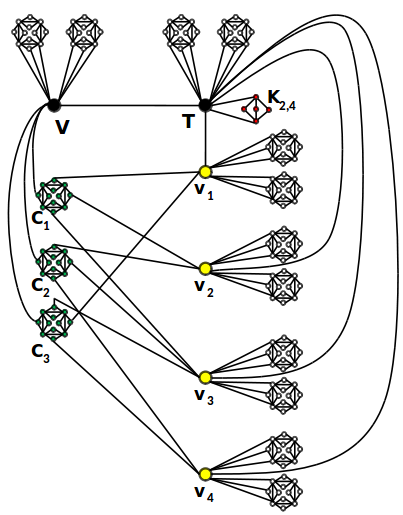
\includegraphics[width=6.5cm]{./img/exemploGrafoGFSBPO4.png}
\caption{The $G_{F}$ graph corresponding to formula $F=(x_1+ x_2+ x_3) \wedge  (x_2+ x_3+ x_4 )\wedge  (x_3 + x_1 + x_4 )$}
\label{fig:exemploGrafoGF}
\end{figure}


\begin{lemma}\label{lem:ida}
Given a satisfiable instance $F$ of {\sc Positive (1 in 3)-3SAT}, the graph $G_F$ constructed from $F$ according to Definition~\ref{sec:reducao} admits a $B_{1}$-EPG-Helly representation.
\end{lemma}


% \begin{proof}

% %~\ref{fig:representacaoCaminhos}
% We will use the true pie and false pie structures to represent the \textit{clause gadgets} $ G_C$, but the construction could also be done with the frame structure without loss of generality, see Figure~\ref{fig:falseAndTruePie}.  


% \begin{figure}[htb]
  \centering
%segundo bloco de figuras
  \begin{tabular}{c c c }
    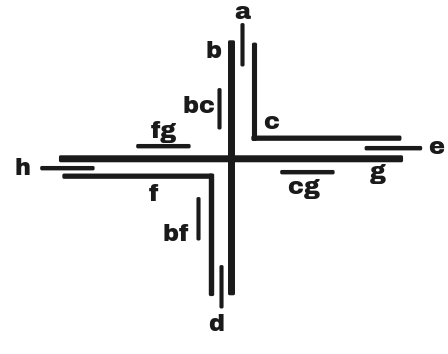
\includegraphics[width=4.5cm]{./img/falsePie.png}  %\label{fig:falsePie} 
    & &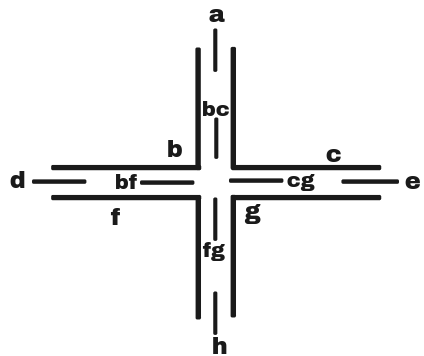
\includegraphics[width=4.5cm]{./img/truePie.png} %\label{fig:truePie}
    \\%[\abovecaptionskip]
    {\footnotesize (a) Based in false pie}  & &  {\footnotesize(b) Based in true pie}\\
  \end{tabular}
  \caption{Single bend representations of a clause gadget isomorph to graph $H$
  %, see Figure~\ref{fig:gadgetBase}
  }\label{fig:falseAndTruePie}
\end{figure} 

% The \textit{variable gadgets} will be represented by structures as of the Figure~\ref{fig:gadgetVariavel}.

% \begin{figure}[htb]	
\center%6.3
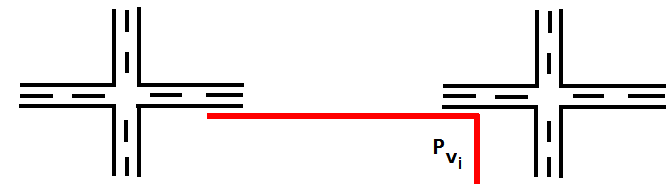
\includegraphics[width=8cm]{./img/gadgetVariavel.png}
%clausulaGadgetGFCompletaSBPO
\caption{Single bend representation of a variable gadget}
\label{fig:gadgetVariavel}
\end{figure}


% The \textit{base gadget} will be represented by the structure of the Figure~\ref{fig:gadgetBaseSingleBend}.

% \begin{figure}[htb]	
\center%6.3
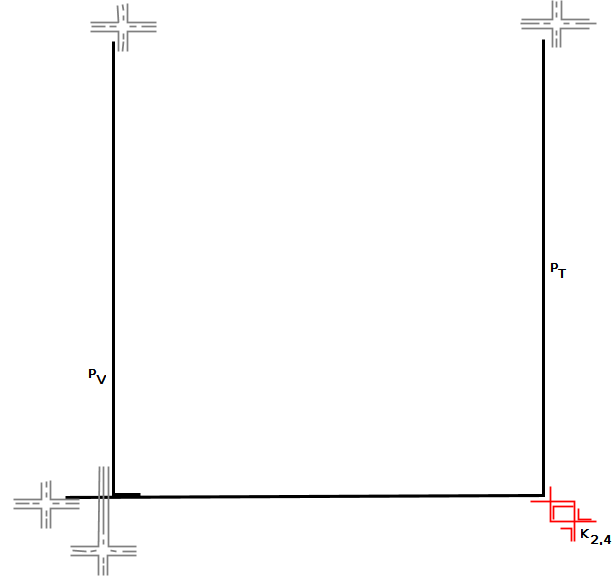
\includegraphics[width=10cm]{./img/gf2.png}
%clausulaGadgetGFCompletaSBPO
\caption{Single bend representation of the base gadget}
\label{fig:gadgetBaseSingleBend}
\end{figure}


% It is easy to see that the representations of the clause gadgets, variable gadgets, and base gadgets are all $B_1$-EPG-Helly. Now we need to describe how these representations can be combined in order to construct a single bend representation $R_{G_F}$.

% Given an assignment $A$ that satisfies $F$, we can construct a  $B_{1}$-EPG-Helly representation $R_{G_F}$. First we will fix the representation structure of the base gadget in the grid to guide the single bend representation, see Figure~\ref{fig:gadgetBaseSingleBend}. Next we will insert the variable gadgets with the following rule: if the  variable $x_i$ related to the path $p(v_i)$ had assignment \textit{True}, then the adjacency between the path $p(v_i)$ with $p(T)$ is horizontal, and vertical otherwise. For example, for an assignment $A=\{x_1=False; x_2=False;x_3=True; x_4=False\}$  to variables of the formula $F$ that generated the gadget $G_F$ of the Figure~\ref{fig:exemploGrafoGF}, it will give us a single bend representation (base gadget + variables gadget) according to the Figure~\ref{fig:gadgetBasePlusVariables}(a). 

%  When a formula $F$ of {\sc Positive (1-in-3)-3sat} has clauses whose format of assignment is $(False, True, False)$ or $(False, False, True)$ then we will use false pie to represent these clauses, but when the clause has format $(True, False, False)$ we will use true pie to represent this clause. To insert a \textit{ clause gadget} $G_{C}$, we introduce a horizontal line $l_{h}$ in the grid between the horizontal lines used by the paths for the two false variables in $ C $. Then we connect the path $p(d_{c_i})$ of $G_{C_i}$ in $p(V)$ vertically using the bend of $p(d_{c_i})$. However, we introduce a vertical line $ l_{v}$ in the grid, between the vertical line of the grid used by $p(V)$ and the path to the true variable in $C_i$, i.e. between $p(V)$ and the path of the true variable $x_j \in C_i$. Where $l_{h}$ and $l_{v}$ cross, to insert the center of the  \textit{clause gadget} as can be seen in Figure~\ref{fig:gadgetOnePie}(b). A complete construction of this single bend representation for the $G_F$ can be verified in 
% Figure~\ref{fig:gadgetFormulaCompletaPies}.%~\ref{fig:clausulagadgetgf}. 

% \begin{landscape}
% % \begin{figure}[htb]	
% \center%6.3
% 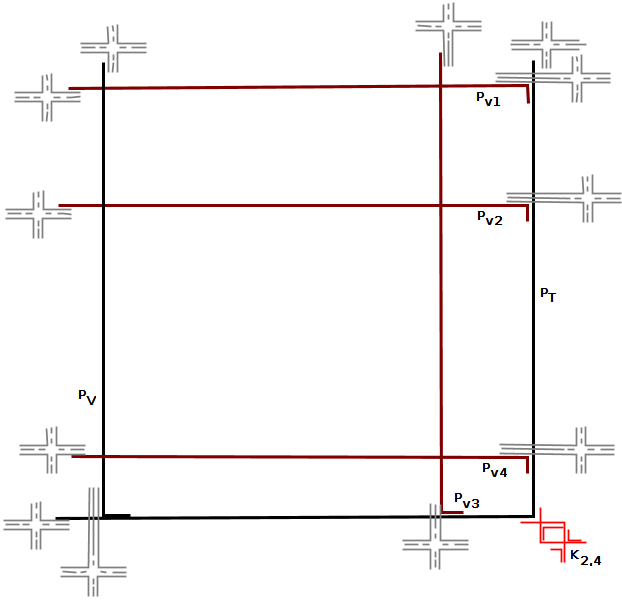
\includegraphics[width=10cm]{./img/gf3.png}
% %clausulaGadgetGFCompletaSBPO
% \caption{Single bend representation of the base and variables gadgets associated with the assignment $x_1=False, x_2=False, x_3=True, x_4=False$ }
% \label{fig:gadgetBasePlusVariables}
% \end{figure}
\begin{figure}[h]
  \centering
%segundo bloco de figuras
  \begin{tabular}{p{6cm} p{6cm}}
   \centering 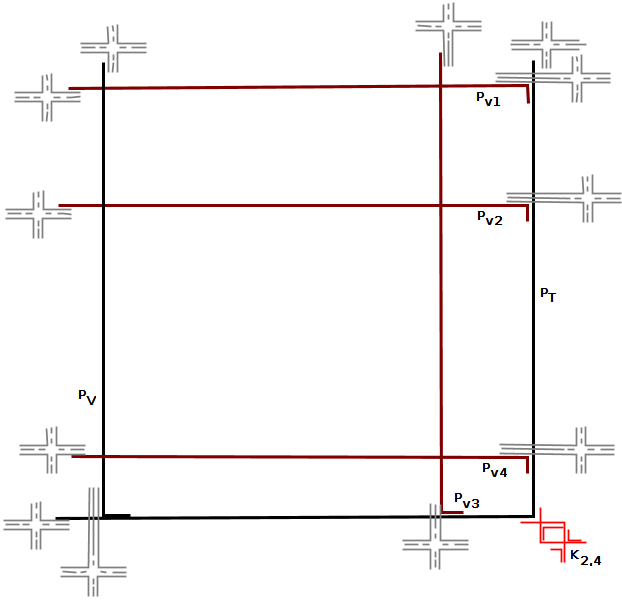
\includegraphics[width=6cm, left]{./img/gf3.png} & 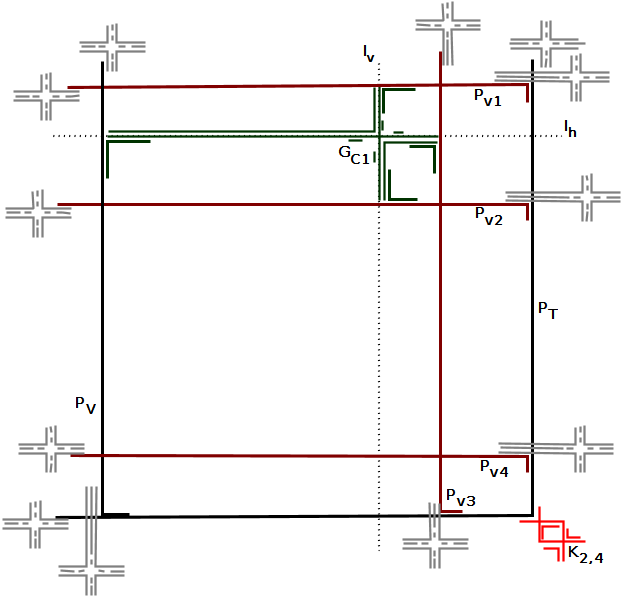
\includegraphics[width=6cm, left]{./img/formulaCompletaGFonePiePlusLines.png} \\  
  [\abovecaptionskip]
    \footnotesize \centering (a) Representation with omitted clause gadgets & \footnotesize(b) Representation with  $G_{C_1}$  associated with the clause $(x_1+x_2+x_3)$ in highlighted \\
%    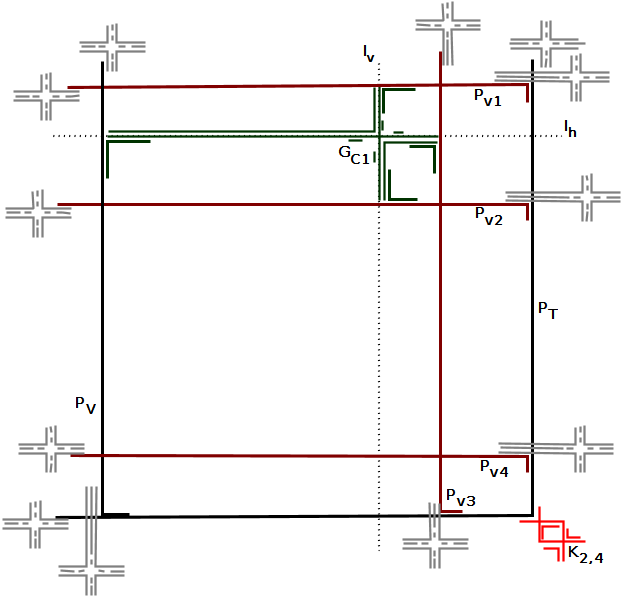
\includegraphics[width=10cm]{./img/formulaCompletaGFonePiePlusLines.png}
%   \\
%     \footnotesize(b) Representation with  $G_{C_1}$  associated with the clause $(x_1+x_2+x_3)$ in highlighted \label{fig:gadgetOnePie}
% \\
  \end{tabular}

 \caption{Single bend representation of the base and variables gadgets associated with the assignment $x_1=False, x_2=False, x_3=True, x_4=False$} \label{fig:gadgetOnePie} \label{fig:gadgetBasePlusVariables}
\end{figure}
% \end{landscape}


% \begin{figure}[htb]	
\center%6.3
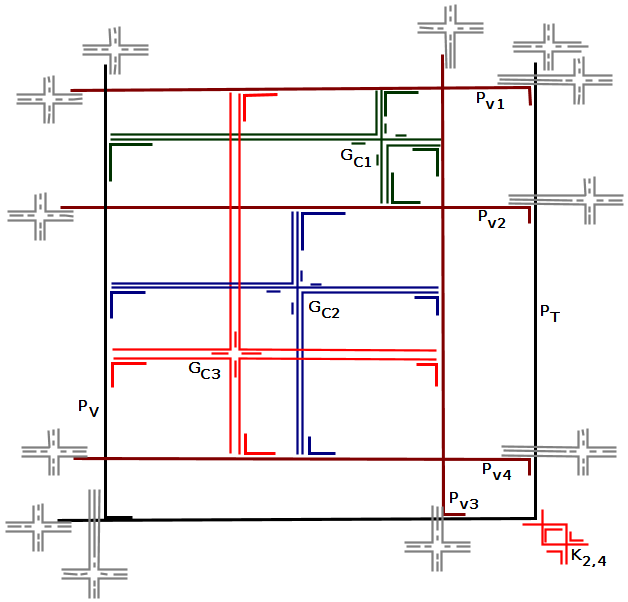
\includegraphics[width=10cm]{./img/formulaFGCompletaPies.png}
%clausulaGadgetGFCompletaSBPO
\caption{Single bend representation of $G_F$}
\label{fig:gadgetFormulaCompletaPies}
\end{figure}


% Note that when we join all these representations of gadgets that form $ R_{G_F} $ we do not insert more bends in paths that had already bend then the representation is necessarily  $ B_1$-EPG. Let us show that it satisfies the Helly property. 

% A simple way to check that $ R_{G_F} $ satisfies the Helly property  is to note that the particular graph $G_F$ never forms triangles between variable, clause, and base gadgets. Thus, any triangle of $G_F$ is inside a variable, clause or base gadget. As we only use $B_1$-EPG-Helly representations of such gadgets, $ R_{G_F} $ is a $B_1$-EPG-Helly representation of $G_F$.
% $\square$ \end{proof}

%\cleardoublepage
%\newpage

Next, we consider the converse. Let a $B_1$-EPG-Helly representation $R$ of $G_F$.

%To complete the proof of $NP$-hardness we will  present some considerations related with the single bend representation of gadgets that form the graph $G_F$. The way all gadgets can be drawn makes it possible to recover the formula that generated $G_F$ and a $True-$assignment for it. The following proofs help us understand the construction of a representation to $G_F$.  

%\subsection{Representations for the graph $C_4$}

\begin{definition}
Let $H$ be the graph shown in Figure~\ref{fig:gadgetBase}, such that the 4-cycle $H[\{b, c, f, g \}]$ corresponds in $R$ to a false pie or true pie, then:

\begin{itemize}
\item the \emph{center} is the unique grid-point of this representation which is contained in every path representing 4-cycle $ \{b, c, f, g \}$; \label{lab:lab1}

\item a \emph {central ray} is an edge-intersection  between two of the paths corresponding to vertices  $ b, c, f, g$, respectively.
\end{itemize}
\end{definition}


Note that every $B_1$-EPG representation of a $C_4$ satisfies the Helly property, see Lemma~\ref{lem:representacaoC4}, and triangles have $B_1$-EPG representations that satisfy the Helly property, e.g. the one shown in Figure~\ref{fig:trianguloepgRepresentacao}(b). The graph $H$ is composed by a 4-cycle  $C_4^{H}=H[b, c, f, g]$ and eight cycles of size 3.%, which are $(a,b,c);$ $(b,c,bc);$ $(c,e,g);$ $(c,g,cg);$ $(f,g,h);$ $(f,g,fg);$ $(b,d,f);$ $(b,f,bf).$

As $C_4^{H}$ has well known representations (see in Lemma~\ref{lem:representacaoC4}), then we can start drawing the $B_{1}$-EPG-Helly representation of $H$ from these structures.  Figures~\ref{fig:falsepietruepieframe} shows possible representations for $H$.

%(a), ~\ref{fig:falsepietruepieframe}(b) and ~\ref{fig:falsepietruepieframe}(c) present 3 possible representations of $H$.


If $C_4^{H}$ is represented by pie, then the paths $p(b), p(c), p(f), p(g)$ share a central point of the representation. On the other hand, if $C_4^{H}$ is represented by a frame then the bends of the 4 paths corresponding to the four distinct corners of a rectangle, i.e. all path representing the vertices of $C_4^{H}$ have distinct bend points, see~\cite{golumbic2009}.

Next we examine the use of the frame structure.

%Due asymmetric representations, the frame structure needs to be studied in more detail. Next we will show some constraints of this structure. % in which allow us to consider it. %as gadget in the demonstration.

\begin{proposition}\label{lem:direcoesdiferentes}
In a $B_1$-EPG representation of a $C_4$ isomorphic to a frame, every path $P_i$ that represents a vertex of the $C_4$ intersects exactly two other paths $P_{i-1}$ and $P_{i+1}$ of the frame, so that one of the intersections is horizontal and the other is vertical. %where one of them is vertical and another is a horizontal intersection.
\end{proposition}

% \begin{proof}
% The proof is immediate.
% $\square$ \end{proof}

\begin{proposition}\label{lem:mesmaretasuporte}
Given a $B_1$-EPG-Helly representation of a graph $G$ that has an induced $C_4$ whose representation is isomorphic to a frame. If there is a vertex $v$ of $G$, outside this $C_4$, that is adjacent to exactly two consecutive vertices of this $C_4$, then the path representing $v$ shares at least one common edge-intersection with the paths representing both of these vertices.% of $v$ into such $C_4$.  
\end{proposition}

% \begin{proof}
% By assumption, $G$ has a triangle containing $v$ and two vertices of a $C_4$. Therefore the path representing $v$ shares at least one common edge intersecting with the paths representing these neighbors, otherwise the representation does not satisfy the Helly property.
% $\square$ \end{proof}

%\cleardoublepage

By Proposition~\ref{lem:direcoesdiferentes} and Proposition~\ref{lem:mesmaretasuporte} we can conclude that for every vertex $v_i \in V(H)$ such that $v_i \neq V(C_4^{H})$, when we use a frame to represent the $C_4^{H}$, $p(v_i)$ will have at least one common edge-intersection to a pair of paths representing its neighbor vertices of $H$. 
Figure~\ref{fig:falsepietruepieframe}(c) presents a possible $B_{1}$-EPG-Helly representation of $H$. 
Note that we can apply rotations and mirroring operations, while maintaining it as a $B_1$-EPG-Helly representation of $H$.
%On this $B_{1}$-EPG-Helly representation presented we can apply rotation and mirroring operations, because these operations do not change the structure. We can also a change the direction of the bend (see Figure~\ref{fig:falsepietruepieframe}(c) and Figure~\ref{fig:outraRepresentacaoFrame}), but also adjust other paths if needed, so as to not change the intersections between the paths.

\begin{definition}
In a single bend representation of a graph $C_4$ isomorphic to a frame, the paths that represent consecutive vertices in the $C_4$ are called \emph{consecutive paths} and the segment that corresponds to the intersection between two consecutive paths is called \emph{side intersection}.  
\end{definition}

\begin{lemma}\label{lem:2vertical2horizontal}
In any single bend minimal representation of a graph isomorphic to $H$, there are two paths in $\{p(a), p(e), p(d), p(h) \}$ that have horizontal directions and the other two paths have vertical directions.
\end{lemma}

% \begin{proof}
% If the $C_4^{H} = [b,c,f,g]$ is  represented by a true pie or false then each path of $C_4^{H}$ share two central rays with two other paths of $C_4^{H}$, where each central rays corresponds to one pair of consecutive vertices in $C_4^{H}$.

% As the vertices $a, e, d $ and $ h$ are adjacent to pairs of consecutive vertices in $C_4^{H}$ so the paths $p(a), p(e), p(d)$ and $p(h)$ have to be positioned in each one of the different central rays,  2 are horizontal  and 2 are vertical.

% If the $C_4^{H}$ is  represented by a frame then each path of the $C_4^{H}$ has a bend positioned in  the corners of the frame. In the frame, the adjacency relationship of pairs of consecutive vertices in the $C_4^{H}$ is represented by the edge-intersection of the paths that constitute the frame. Thus, since a frame has two parts in the vertical direction and two parts in the horizontal direction, then there are two paths in $\{p(a), p(e), p(d), p(h)\}$ that have horizontal direction and two that have vertical direction.
% $\square$ \end{proof}

\begin{corollary} \label{coro:paresMesmoSegmento}
In any single bend minimal representation of a graph isomorphic to $H$, the following paths are on the some central ray or side intersection: $p(a)$ and $p(bc)$; $p(e)$ and $p(cg)$; $p(h)$ and $p(fg)$; $p(d)$ and $p(bf)$.

% \begin{itemize}
% \item $p(a)$ and $p(bc)$;
% \item $p(e)$ and $p(cg)$;
% \item $p(h)$ and $p(fg)$;
% \item $p(d)$ and $p(bf)$.
% \end{itemize}
\end{corollary}

\begin{figure}[htb]
  \centering
%segundo bloco de figuras
  \begin{tabular}{c c c c c }
    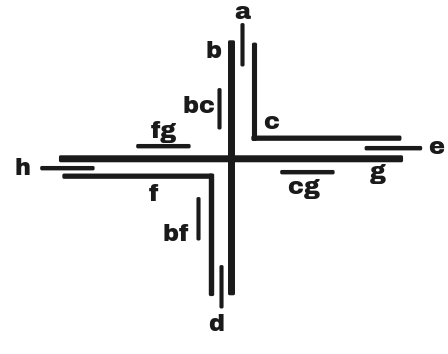
\includegraphics[width=4cm]{./img/falsePie.png}  %\label{fig:falsePie} 
    & &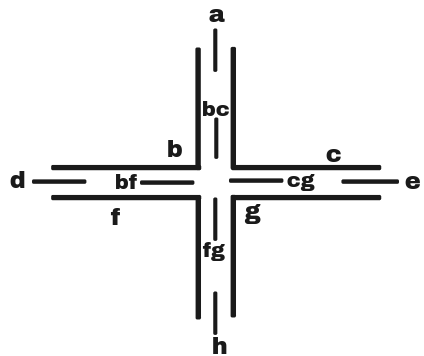
\includegraphics[width=4cm]{./img/truePie.png} %\label{fig:truePie}
    & &
 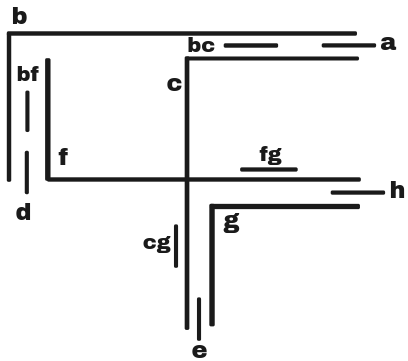
\includegraphics[width=4cm]{./img/frame.png} \\%[\abovecaptionskip]
    {\footnotesize (a) Based in false pie}  & &  {\footnotesize(b) Based in true pie} & & {\footnotesize (c) Based in frame} %\label{fig:frame}
  \end{tabular}
  \caption{Different single bend representations of the  graph $H$ using a false pie (a), a true pie (b) and a frame (c) for representing  $C_4^{H}$}\label{fig:falsepietruepieframe}
\end{figure} 

\begin{figure}[htb]	
\center%6.3
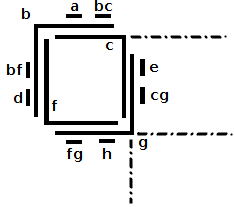
\includegraphics[width=4cm]{./img/outraRepresentacaoFrame3.png}
\caption{A frame representation where the bend of dashed paths change directions}
\label{fig:outraRepresentacaoFrame}
\end{figure}

\begin{definition}
Consider a graph $G$ and a vertex $v \in V(G)$. If in a $B_1$-EPG representation of $G$ the two bend edges (or one extremity edge) of the path $p(v)$ intersects other paths, then we say that $p(v)$ has an \emph{obstructed bend (or extremity)}. 
In addition, given a $B_1$-EPG representation of $G$ where $p(v)$ has an obstructed bend (or extremity), we say that a subset of paths \emph{obstructs} a bend edge (or a extremity edge) of $p(v)$ if it intersects such an edge. 
\end{definition}


\begin{remark} \label{fact:k24facts}
In every single bend representation of a $K_{2,4}$, the path representing each vertex of the larger part has its bend in a false pie (claim in~\cite{daniel2014b} and reasoning in~\cite{Asinowski2009}).
\end{remark} %fac


% \begin{lemma}\label{lem:obstrucao}
% In any single bend representation of the graph $G'$ presented in Figure~\ref{fig:extremidadeDobraObstruida}(a), the path $p(x)$ has obstructed extremities and bend.
% \end{lemma}

% \begin{proof}
% Consider $G'$ consisting of a vertex $x$, two graphs isomorphic to $H$, $ H_1 $ and $ H_2 $, and a bipartite graph $K_{2,4}$, such that: $x$ is a vertex of the largest stable set of the $K_{2,4}$; $x$ is adjacent to an induced cycle of size 3 of $H_1$, $C_3^{H_1}$ and to an induced cycle of size 3 of $H_2$, $ C_3^{H_2}$, see Figure~\ref{fig:extremidadeDobraObstruida}(a).

% We know that the paths belonging to the largest stable set of a $K_{2,4}$ always will bend into a false pie, see Fact~\ref{fact:k24facts}. Since $p(x)$ is part of the largest stable set of the $K_{2,4}$, then $p(x)$ has an \emph {obstructed bend}, see Figure~\ref{fig:extremidadeDobraObstruida}(b). 

% The vertex $x$ is adjacent to $ C_{3}^{H_1}$ and $ C_3^{H_2}$, so that its path $ p(x) $ intersects the paths representing them.  But in a single bend representations of a graph isomorph to $H$ there are pairs of paths that always are on some segment of a central ray or a side intersection, see Corollary~\ref{coro:paresMesmoSegmento}, and the representation of $C_{3}^{H_1}$ ( similarly $C_3^{H_2})$ has one these paths. Therefore, there is an edge in the set paths that represent ${H_1}$ ( similarly in ${H_2}$) that has a intersection of 3 paths representing $ C_{3}^{H_1}$ (and $ C_3^{H_2}$), otherwise the representation would not be Helly, and there is one other different edge in the some central ray or side intersection that contains three other paths and one of them is not in set paths  $C_{3}^{H_1}$ ( similarly $C_3^{H_2})$. Thus in a single bend representation of $G'$, the paths that represent  $C_{3}^{H_1}$ ( similarly $C_3^{H_2})$ must intersect in a bend edge or an extremity edge of $p(x)$, because $p(x)$ intersects only one of set paths that are on some central ray or side intersection where  $C_{3}^{H_1}$ ( similarly $C_3^{H_2})$ is. As the bend of $G'$ is already obstructed by structure of $K_{2,4}$, then ${H_1}$ ( similarly in ${H_2}$) must be positioned at an extremity edge of $p(x)$. This implies that $ p(x) $ has a condition of \emph{obstructed extremities}, see Figure~\ref{fig:extremidadeDobraObstruida}(b).
% \begin{figure}[h]
  \centering
  \begin{tabular}{p{6cm} p{0.5cm} p{6cm}}
     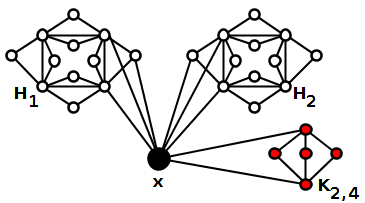
\includegraphics[width=5cm, center]{./img/grafoDobraExtremidadeObstruida2.png} &  &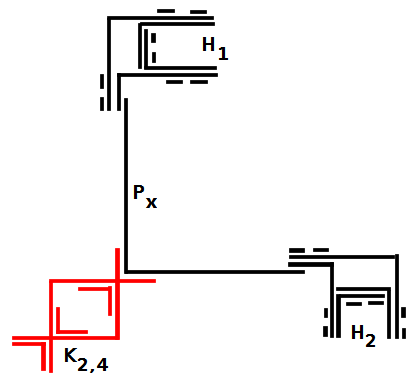
\includegraphics[width=5cm, center]{./img/extremidadeDobraObstruida4.png}  \\%[\abovecaptionskip]
    \footnotesize \centering (a) The graph $G'$& & \footnotesize \centering (b)A $B_1$-EPG representation of $G'$%\\
 %   &&
  \end{tabular}
 \caption{The sample of  obstructed extremities and bend.}\label{fig:extremidadeDobraObstruida}
\end{figure}
% $\square$ \end{proof}




\begin{definition}
We say that a segment $s$ is \emph{internally contained} in a path $p(x)$ if $s$ is contained in $p(x)$, and it does not intersect a relevant edge of $p(x)$. 
\end{definition}

% \begin{fac}
% In a single bend representation of a graph, if a path $p(y)$ has an obstructed bend and obstructed extremities, and some path $p(x)$ intersects $p(y)$, but does not intersect paths that obstruct the extremities and the bend edges of $p(y)$, then the intersection between $p(x)$ and $p(y)$ is internally contained into $p(y)$. 
% \end{fac}


\begin{lemma}\label{lem:volta}
If a graph $G_F$, constructed according to Definition~\ref{sec:reducao}, admits a $B_1$-EPG-Helly representation, then the associated CNF-formula $F$ is a yes-instance of {\sc Positive (1 in 3)-3sat}.
\end{lemma}

% \setcounter{proof}{3}
% \begin{proof}
% Suppose that $G_F$ has a $B_1$-EPG-Helly representation, $R_{G_F}$.  From $R_{G_F}$ we will construct an assignment that satisfies $F$. 

% First, note that in every single bend representation of a $K_{2,4}$, the path of each vertex of the greater stable set, in particular $p(T)$ (in $R_{G_F}$), has bends contained in a false pie (see Fact~\ref{fact:k24facts}). 


% The vertex $T$ is adjacent to the vertices of a triangle of $G_{B1}$ and $G_{B2}$. As the $K_{2,4}$ is positioned in the bend of $p(T)$, then in $R_{G_F}$ the representation of $G_{B1}$ and $G_{B2}$ are positioned at the extremities of $p(T)$, see Lemma~\ref{lem:obstrucao}.   


% Without loss of generality assume that $p(V) \cap p(T)$ is a horizontal segment in $R_{G_F}$.

% We can note in $R_{G_F}$ that: the number of paths $p(d)$ with segment internally contained in $p(V)$ is the number of clauses in $F$; the intersection between each $p(a), p(e), p(h)$ in the gadget clause and each path $p(v_j)$ indicates the variables composing the clause. Thus, we can assign to each variable $ x_{j}$ the value \textit{True} if the edge intersecting $p(v_j)$ and $p(T)$ is horizontal, and \textit{False} otherwise. 


% In Lemma~\ref{lem:2vertical2horizontal} it was shown that any minimal $B_1$-EPG representation of a clause gadget has two paths in $\{p(a), p(d), p(e), p(h)\}$ with vertical direction and the other two paths have horizontal direction. Since $p(d)$ intersects $p(V)$, it follows that in a single bend representation of $G_F$ we must connect two of these in order to represent a false assignment, and exactly one will represent a true assignment. Thus, from $R_{G_F}$ we construct an assignment to $F$ such that every clause has exactly one variable with a true value.  
% $\square$ \end{proof}

\begin{theorem}
{\sc $B_{1}$-EPG-Helly graph recognition} is $NP$-complete.
\end{theorem}
\begin{proof} %\textbf{Proof}.
By Theorem~\ref{teo:nppertinencia} and Lemmas~\ref{lem:ida} and~\ref{lem:volta}.
$\square$ \end{proof}

We say that a $k$-apex graph is a graph that can be made planar by the removal of $k$ vertices. In addition, a $d$-degenerate graph is a graph in which every subgraph has a vertex of degree at most $d$.

\begin{corollary}\label{coro:2apexAnd3degenerate}
{\sc $B_{1}$-EPG-Helly graph recognition} is $NP$-complete on $2$-apex and $3$-degenerate graphs.
\end{corollary}

Some of the vertices of $G_F$ have highly constrained $B_1$-EPG representations. Vertex $T$ has its bend	and both extremities	obstructed	by its neighbors in	$G_{B1}$, $G_{B2}$ and in the $K_{2,4}$
subgraphs. Vertex $V$ and each variable vertex $v_i$ must have one of its segments internally contained in $T$, and also have its extremities and bend obstructed.  Therefore, vertex $V$ and each
variable vertex have only one segment each that can be used in an EPG
representation to make them adjacent to the clause gadget. The direction of
this segment, being either horizontal	or vertical, can be used to represent
the true or false value	for the	variable.
The clause gadgets, on the other hand, are such that exactly two of its
adjacencies to the variable vertices and to $V$ can be realized with a
horizontal intersection whereas  the other two must be realized with a
vertical intersection. If we consider the direction used by $V$ as a
truth assignment, we get that exactly one of the variables in each clause
will be	true in	any possible representation of $G_F$. Conversely, it is	fairly
straightforward to obtain a $B_1$-EPG representation for $G_F$ given a truth assignment	for
the formula $F$.

\bibliographystyle{splncs04}
\bibliography{refs}

% \begin{proof}
% It is easy to see that the graphs constructed according to Definition~\ref{sec:reducao} are $3$-degenerate.
% As {\sc Positive (1 in 3)-3SAT} remains NP-complete when the incidence graph of $F$ is planar~\cite{mulzer2008minimum}, from an instance $F$ of {\sc Planar Positive (1 in 3)-3SAT}, by using a planar embedding of the incidence graph of $F$, one can observe that by removing $V$ and $T$ from $G_F$ we obtain a planar graph. Thus, $G_F$ is 2-apex. 
% $\square$ \end{proof}



\newpage

\section*{Appendix}

We describe the proofs that have been omitted in the text, as well as some additional comments.


%\hspace{0.3cm}
\begin{lemma*} \textbf{Lemma} \ref{lem:todoGrafoEpgHelly}:
 Every graph is an EPG-Helly graph.
 \end{lemma*}
 %\setcounter{proof}{1}
 
  \begin{proof}  %\textbf{Proof} 
  \ref{lem:todoGrafoEpgHelly}:
  Let $G$ be a graph with $n$ vertices $v_1, v_2, \dots, v_n$ and $\mu$ maximal cliques $C_1, C_2, \dots , C_{\mu }$. We construct an EPG-Helly representation of $G$, using a grid $Q$ of size $(\mu \times 2n)$. The lines correspond to the maximal cliques and are numbered $1, 2, \dots , \mu$. Each vertex $v_j$ corresponds to the pair of columns $j, j+n$. Each maximal clique $C_i$ is mapped into an edge $(i,n), (i,n+1)$. Each path $P_j$ contains all edges $(i,n), (i,n+1)$ corresponding to the maximal cliques $C_i$ containing $v_i$.
  
  Moreover, two distinct paths $P_j,P_k$ intersect at the edges corresponding to the maximal cliques containing $v_j,v_k$.
  
  Let $v_j \in V(G)$, consider the maximal cliques containing $v_j$ in ascending order of their indices. The path $P_j$ representing $v_j$, start at vertex $(1,j)$ of $Q$ and descends column $j$ until $(i,j)$, where $C_i$ is the first clique containing $v_j$ then $P_j$ bends at vertex $(i,j)$ and proceeds to the right, travesses edge $(i,n), (i,n+1)$ representing $C_i$. Then $P_j$ proceeds further on line $i$ until reaching vertex $(i, j+n)$, where it bends again, descending column $j+n$ until reaching vertex $(l,j), l>i$, where $C_l$ is the next maximal clique containing $v_j$ where it bends again. It proceeds in line $l$, travessing edge $(l,n),(l,n+1)$, and so on, until all edges of $Q$ corresponding to the maximal cliques containing $v_j$ have been travessed by $P_j$.   
  
It follows that two distinct paths, $P_j$ and $P_q$, intersect exactly at the lines corresponding to the maximal cliques containing both $v_j$ and $v_q$.  
  $\square$ \end{proof}
 
 Figure~\ref{fig:gradeDemonstracao} shows the grid $Q$ and the path $P_2$ corresponding to the vertex $v_2 \in V(G)$, contained in maximal cliques $C_2, C_4$ and $C_5$ of $G$.
 
  \begin{figure}[htb]	
\center%6.3
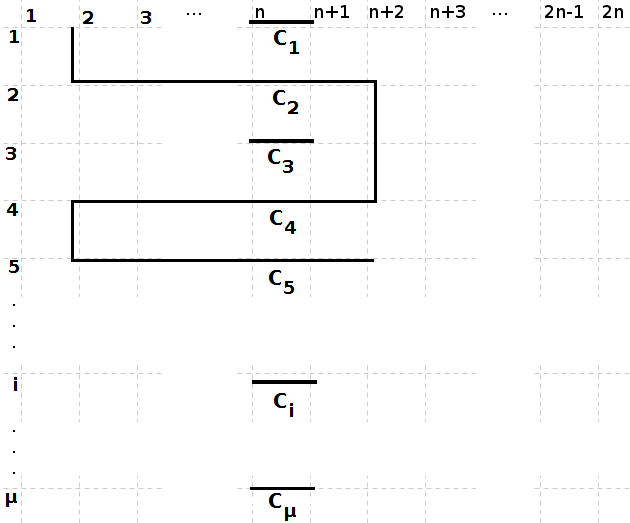
\includegraphics[width=8cm]{./img/grade3.png}
%clausulaGadgetGFCompletaSBPO
\caption{Representation of the path $P_2$ corresponding to vertex $v_2$ contained in cliques $C_2, C_4$ and $C_5$}
\label{fig:gradeDemonstracao}
\end{figure}
 

\begin{lemma*}\textbf{Lemma} \ref{lem:octaedronaohelly}:
The octahedral graph $O_3$ has a unique minimal  $ B_1$-EPG representation.%, without considering isomorphisms.
\end{lemma*}

\begin{proof}
%\textbf{Proof} 
\ref{lem:octaedronaohelly}:
The octahedral graph $ O_3 $ has in its constitution induced cycles of size 4 ($ C_4$'s). 
Take an induced $ C_4 $ subgraph  of the octahedral $ O_3 $. The pairs of non-adjacent vertices of the induced $C_4$ are false twins whose neighborhoods are the remaining of vertices of the induced $C_4$. Each of the vertices outside the $C_4$ are adjacent to all vertices of the $C_4$. Thus, if in a $ B_1$-EPG representation of $C_4$, the $ C_4 $ is represented as a frame, no single bend path can simultaneously intersect the 4 paths representing the vertices of the induced $ C_4 $. Therefore, we conclude that the frame structure can not be part of a $ O_3 $ representation.

With the same reasoning, take a $ B_1$-EPG representation of $C_4$ where the induced $ C_4 $ subgraph is represented as true pie or false pie. When adding the false twin vertices, which are neighbors of all vertices of $ C_4 $ taken from $ O_3 $, both representations converge to the structure represented in Figure~\ref{fig:octaedro}(b). 
$\square$ \end{proof}

%\begin{figure}[h]
  \centering
  
%segundo bloco de figuras
  \begin{tabular}{@{}c@{} p{1.5cm} @{}c@{} }
   \centering 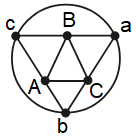
\includegraphics[width=2.5cm]{./img/octaedro.png} & &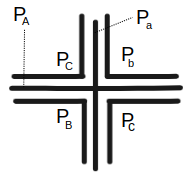
\includegraphics[width=2.9cm]{./img/representacaoOctaedro.png}  \\[\abovecaptionskip]
    \footnotesize \centering (a) The octahedral $O_3$ graph  & &  \footnotesize(b) $B_1$-EPG representation of the graph $O_3$
  \end{tabular}

 \caption{The octahedral $O_3$ graph and its  $B_1$-EPG representation}\label{fig:octaedro}
\end{figure}

\begin{lemma*}\textbf{Lemma} \ref{lem:verify1}:
Each path $P_i$ can be determined in polynomial time, from the considered sequence of edge.
\end{lemma*}

\begin{proof}%\textbf{Proof} 
\ref{lem:verify1}: 
It is easy to verify that~\ref{it:bullet1} is true, consider the sequence of relevant edges of some path $P_i\in \mathcal{P}$. Start from an extremity edge of $P_i$. Let $t$ be the line (column) containing the last considered relevant edge. The next relevant edge $e'$ in the sequence, must be also contained in line (column) $t$. If $e'$ is an extremity edge, the process is finished and the path has been determined. It contains all edges between the considered relevant edges in the sequence. Otherwise, if $e'$ is a bend edge , the next relevant edge is the second bend edge $e''$ of this same bend, which is contained in some column (line) $t'$. The process continues until the second extremity edge of $P_i$ is located.   

With the above procedure, we can determine in $O(k+|V(G)|)$ time, whether path $P_i$ contains any given edge of the grid $Q$. Therefore, the sequence of relevant edges of $P_i$ uniquely determines $P_i$.
$\square$ \end{proof}


\begin{lemma*}
\textbf{Lemma} \ref{lem:relevantEdges}:
Let $R$ be a $B_k$-EPG-Helly representation of $G$, and $P_1, P_2 \in \mathcal{P}$ paths of $R$. Then $P_1, P_2$ are intersecting paths if and only if they contain a common relevant edge.
\end{lemma*}


\begin{proof}
%\textbf{Proof} 
\ref{lem:relevantEdges}: If $P_1, P_2$ contain a common relevant edge there is nothing to prove. Otherwise, assume that $P_1, P_2$ are intersecting and we show they contain a common relevant edge. Without loss of generality, suppose $P_1, P_2$ intersect at line \textit{i} of the grid, in the  $B_k$-EPG representation $R$. The following are the possible cases that may occur:

\begin{itemize}
\item \textbf{Case 1:} Neither $P_1$ nor $P_2$ contain bends in line \textit{i}. 

Then $P_1$ and $ P_2$  are entirely contained in line \textit{i}. Since they intersect, either $P_1, P_2$  overlap, or one of the paths contains the other. In any these situations, they intersect in a common extremity edge, that is a relevant edge.

\item \textbf{Case 2:} $P_1$ does not contain bends in \textit{i}, but $ P_2$ does contain.

If some bend edge of $P_2$ also belongs to $P_1$, then $P_1, P_2$  intersect in  a relevant edge. Otherwise, since $P_1, P_2$  intersect, the only possibility is that the intersection contains an extremity edge of $P_1$ or $ P_2$. Hence the paths intersect in relevant edge.  

\item \textbf{Case 3:} Both $P_1$,  $P_2$ contain bends in \textit{i}

Again, if the intersection occurs in some bend edge of $P_1$  or $P_2$, the lemma follows. Otherwise, the same situation as above must occur, that is $P_1, P_2$  must intersect in same extremity edge.
 
\end{itemize}
In any of the cases, $P_1$ and $P_2$ intersect in some relevant edge.
$\square$ \end{proof}


\begin{lemma*}\textbf{Lemma} \ref{lem:ida}:
Given a satisfiable instance $F$ of {\sc Positive (1 in 3)-3SAT}, the graph $G_F$ constructed from $F$ according to Definition~\ref{sec:reducao} admits a $B_{1}$-EPG-Helly representation.
\end{lemma*}


\begin{proof}
%\textbf{Proof} 
\ref{lem:ida}:
%~\ref{fig:representacaoCaminhos}
We will use the true pie and false pie structures to represent the \textit{clause gadgets} $ G_C$, but the construction could also be done with the frame structure without loss of generality, see Figure~\ref{fig:falseAndTruePie}.  


\begin{figure}[htb]
  \centering
%segundo bloco de figuras
  \begin{tabular}{c c c }
    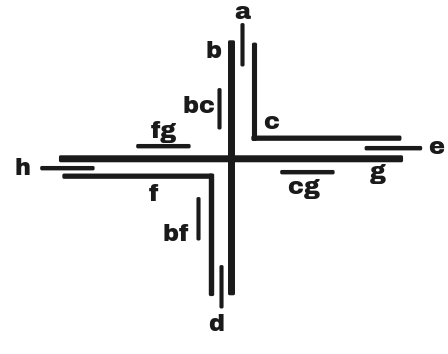
\includegraphics[width=4.5cm]{./img/falsePie.png}  %\label{fig:falsePie} 
    & &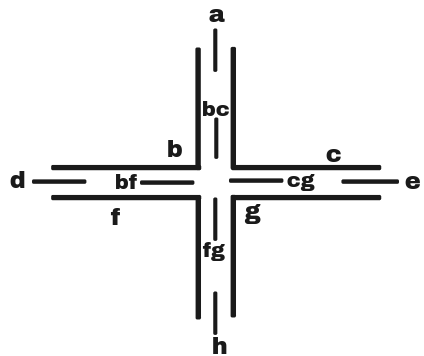
\includegraphics[width=4.5cm]{./img/truePie.png} %\label{fig:truePie}
    \\%[\abovecaptionskip]
    {\footnotesize (a) Based in false pie}  & &  {\footnotesize(b) Based in true pie}\\
  \end{tabular}
  \caption{Single bend representations of a clause gadget isomorph to graph $H$
  %, see Figure~\ref{fig:gadgetBase}
  }\label{fig:falseAndTruePie}
\end{figure} 

The \textit{variable gadgets} will be represented by structures as of the Figure~\ref{fig:gadgetVariavel}.

\begin{figure}[htb]	
\center%6.3
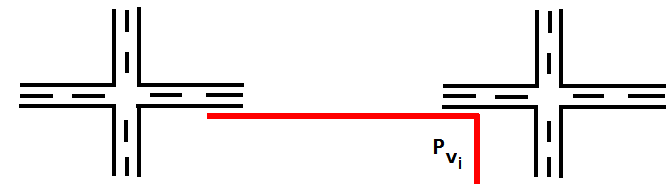
\includegraphics[width=8cm]{./img/gadgetVariavel.png}
%clausulaGadgetGFCompletaSBPO
\caption{Single bend representation of a variable gadget}
\label{fig:gadgetVariavel}
\end{figure}


The \textit{base gadget} will be represented by the structure of the Figure~\ref{fig:gadgetBaseSingleBend}.

\begin{figure}[htb]	
\center%6.3
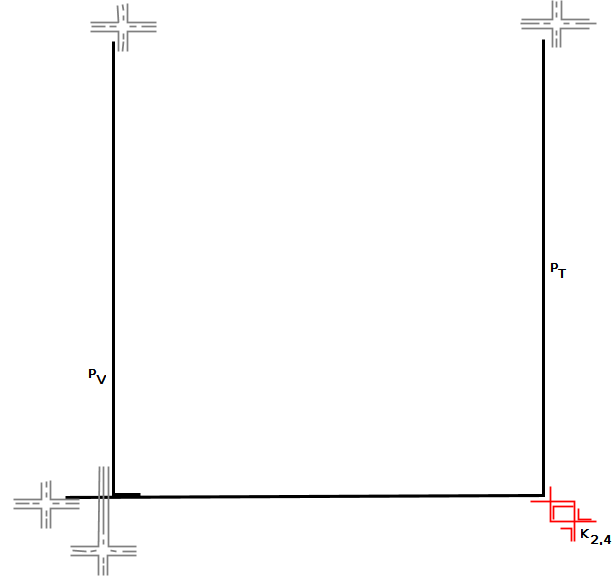
\includegraphics[width=10cm]{./img/gf2.png}
%clausulaGadgetGFCompletaSBPO
\caption{Single bend representation of the base gadget}
\label{fig:gadgetBaseSingleBend}
\end{figure}


It is easy to see that the representations of the clause gadgets, variable gadgets, and base gadgets are all $B_1$-EPG-Helly. Now we need to describe how these representations can be combined in order to construct a single bend representation $R_{G_F}$.

Given an assignment $A$ that satisfies $F$, we can construct a  $B_{1}$-EPG-Helly representation $R_{G_F}$. First we will fix the representation structure of the base gadget in the grid to guide the single bend representation, see Figure~\ref{fig:gadgetBaseSingleBend}. Next we will insert the variable gadgets with the following rule: if the  variable $x_i$ related to the path $p(v_i)$ had assignment \textit{True}, then the adjacency between the path $p(v_i)$ with $p(T)$ is horizontal, and vertical otherwise. For example, for an assignment $A=\{x_1=False; x_2=False;x_3=True; x_4=False\}$  to variables of the formula $F$ that generated the gadget $G_F$ of the Figure~\ref{fig:exemploGrafoGF}, it will give us a single bend representation (base gadget + variables gadget) according to the Figure~\ref{fig:gadgetBasePlusVariables}(a). 

 When a formula $F$ of {\sc Positive (1-in-3)-3sat} has clauses whose format of assignment is $(False, True, False)$ or $(False, False, True)$ then we will use false pie to represent these clauses, but when the clause has format $(True, False, False)$ we will use true pie to represent this clause. To insert a \textit{ clause gadget} $G_{C}$, we introduce a horizontal line $l_{h}$ in the grid between the horizontal lines used by the paths for the two false variables in $ C $. Then we connect the path $p(d_{c_i})$ of $G_{C_i}$ in $p(V)$ vertically using the bend of $p(d_{c_i})$. However, we introduce a vertical line $ l_{v}$ in the grid, between the vertical line of the grid used by $p(V)$ and the path to the true variable in $C_i$, i.e. between $p(V)$ and the path of the true variable $x_j \in C_i$. Where $l_{h}$ and $l_{v}$ cross, to insert the center of the  \textit{clause gadget} as can be seen in Figure~\ref{fig:gadgetOnePie}(b). A complete construction of this single bend representation for the $G_F$ can be verified in 
Figure~\ref{fig:gadgetFormulaCompletaPies}.%~\ref{fig:clausulagadgetgf}. 

%\begin{landscape}
% \begin{figure}[htb]	
% \center%6.3
% 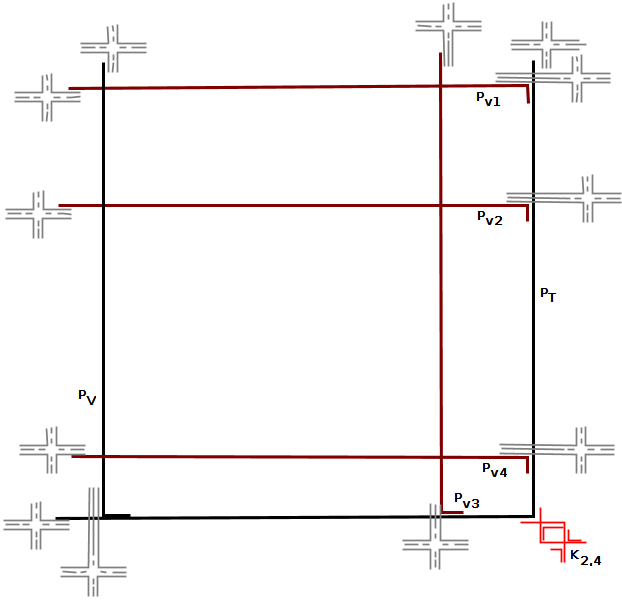
\includegraphics[width=10cm]{./img/gf3.png}
% %clausulaGadgetGFCompletaSBPO
% \caption{Single bend representation of the base and variables gadgets associated with the assignment $x_1=False, x_2=False, x_3=True, x_4=False$ }
% \label{fig:gadgetBasePlusVariables}
% \end{figure}
\begin{figure}[h]
  \centering
%segundo bloco de figuras
  \begin{tabular}{p{6cm} p{6cm}}
   \centering 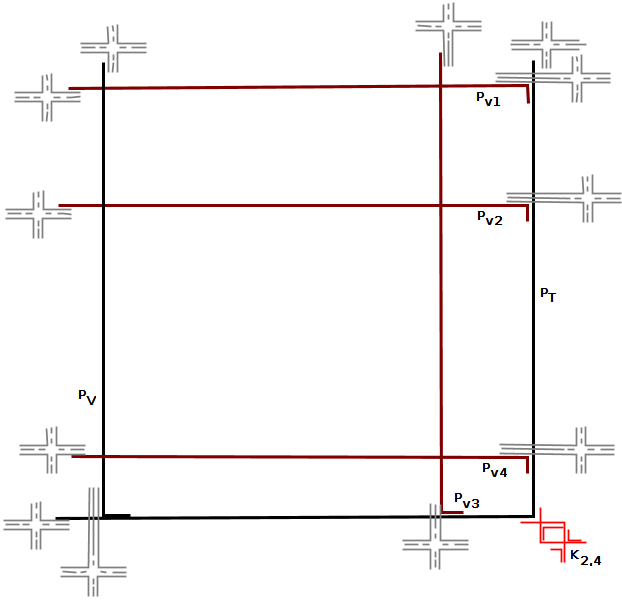
\includegraphics[width=6cm, left]{./img/gf3.png} & \includegraphics[width=6cm, left]{./img/formulaCompletaGFonePiePlusLines.png} \\  
  [\abovecaptionskip]
    \footnotesize \centering (a) Representation with omitted clause gadgets & \footnotesize(b) Representation with  $G_{C_1}$  associated with the clause $(x_1+x_2+x_3)$ in highlighted \\
%    \includegraphics[width=10cm]{./img/formulaCompletaGFonePiePlusLines.png}
%   \\
%     \footnotesize(b) Representation with  $G_{C_1}$  associated with the clause $(x_1+x_2+x_3)$ in highlighted \label{fig:gadgetOnePie}
% \\
  \end{tabular}

 \caption{Single bend representation of the base and variables gadgets associated with the assignment $x_1=False, x_2=False, x_3=True, x_4=False$} \label{fig:gadgetOnePie} \label{fig:gadgetBasePlusVariables}
\end{figure}
%\end{landscape}


\begin{figure}[htb]	
\center%6.3
\includegraphics[width=10cm]{./img/formulaFGCompletaPies.png}
%clausulaGadgetGFCompletaSBPO
\caption{Single bend representation of $G_F$}
\label{fig:gadgetFormulaCompletaPies}
\end{figure}


Note that when we join all these representations of gadgets that form $ R_{G_F} $ we do not insert more bends in paths that had already bend then the representation is necessarily  $ B_1$-EPG. Let us show that it satisfies the Helly property. 

A simple way to check that $ R_{G_F} $ satisfies the Helly property  is to note that the particular graph $G_F$ never forms triangles between variable, clause, and base gadgets. Thus, any triangle of $G_F$ is inside a variable, clause or base gadget. As we only use $B_1$-EPG-Helly representations of such gadgets, $ R_{G_F} $ is a $B_1$-EPG-Helly representation of $G_F$.
$\square$ \end{proof}

\begin{lemma*}\textbf{Lemma} \ref{lem:2vertical2horizontal}:
In any single bend minimal representation of a graph isomorphic to $H$, there are two paths in $\{p(a), p(e), p(d), p(h) \}$ that have horizontal direction and the other two paths have vertical direction.
\end{lemma*}

\begin{proof}%\textbf{Proof} 
\ref{lem:2vertical2horizontal}:
If the $C_4^{H} = [b,c,f,g]$ is  represented by a true pie or false then each path of $C_4^{H}$ share two central rays with two other paths of $C_4^{H}$, where each central rays corresponds to one pair of consecutive vertices in $C_4^{H}$.

As the vertices $a, e, d $ and $ h$ are adjacent to pairs of consecutive vertices in $C_4^{H}$ so the paths $p(a), p(e), p(d)$ and $p(h)$ have to be positioned in each one of the different central rays,  2 are horizontal  and 2 are vertical.

If the $C_4^{H}$ is  represented by a frame then each path of the $C_4^{H}$ has a bend positioned in  the corners of the frame. In the frame, the adjacency relationship of pairs of consecutive vertices in the $C_4^{H}$ is represented by the edge-intersection of the paths that constitute the frame. Thus, since a frame has two parts in the vertical direction and two parts in the horizontal direction, then there are two paths in $\{p(a), p(e), p(d), p(h)\}$ that have horizontal direction and two that have vertical direction.
$\square$ \end{proof}

\begin{pro*} \textbf{Proposition} \ref{lem:mesmaretasuporte}:
Given a $B_1$-EPG-Helly representation of a graph $G$ that has an induced $C_4$ whose representation is isomorphic to a frame. If there is a vertex $v$ of $G$, outside this $C_4$, that is adjacent to exactly two consecutive vertices of this $C_4$, then the path representing $v$ shares at least one common edge-intersection with the paths representing both vertices.% of $v$ into such $C_4$.  
\end{pro*}

\begin{proof} %\textbf{Proof} 
\ref{lem:mesmaretasuporte}:
By assumption, $G$ has a triangle containing $v$ and two vertices of a $C_4$. Therefore the path representing $v$ shares at least one common edge intersecting with the paths representing these neighbors, otherwise the representation does not satisfy the Helly property.
$\square$ \end{proof}


\begin{proposition}
%\textbf{Proposition 4.3}:  
%\ref{lem:obstrucao}:
In any single bend representation of the graph $G'$ presented in Figure~\ref{fig:extremidadeDobraObstruida}(a), the path $p(x)$ has obstructed extremities and bend.
\end{proposition}

\begin{proof} %\textbf{Proof 4.3}: 
Consider $G'$ consisting of a vertex $x$, two graphs isomorphic to $H$, $ H_1 $ and $ H_2 $, and a bipartite graph $K_{2,4}$, such that: $x$ is a vertex of the largest stable set of the $K_{2,4}$; $x$ is adjacent to an induced cycle of size 3 of $H_1$, $C_3^{H_1}$ and to an induced cycle of size 3 of $H_2$, $ C_3^{H_2}$, see Figure~\ref{fig:extremidadeDobraObstruida}(a).

We know that the paths belonging to the largest stable set of a $K_{2,4}$ always will bend into a false pie, see Fact~\ref{fact:k24facts}. Since $p(x)$ is part of the largest stable set of the $K_{2,4}$, then $p(x)$ has an \emph {obstructed bend}, see Figure~\ref{fig:extremidadeDobraObstruida}(b). 

The vertex $x$ is adjacent to $ C_{3}^{H_1}$ and $ C_3^{H_2}$, so that its path $ p(x) $ intersects the paths representing them.  But in a single bend representations of a graph isomorph to $H$ there are pairs of paths that always are on some segment of a central ray or a side intersection, see Corollary~\ref{coro:paresMesmoSegmento}, and the representation of $C_{3}^{H_1}$ ( similarly $C_3^{H_2})$ has one these paths. Therefore, there is an edge in the set paths that represent ${H_1}$ ( similarly in ${H_2}$) that has a intersection of 3 paths representing $ C_{3}^{H_1}$ (and $ C_3^{H_2}$), otherwise the representation would not be Helly, and there is one other different edge in the some central ray or side intersection that contains three other paths and one of them is not in set paths  $C_{3}^{H_1}$ ( similarly $C_3^{H_2})$. Thus in a single bend representation of $G'$, the paths that represent  $C_{3}^{H_1}$ ( similarly $C_3^{H_2})$ must intersect in a bend edge or an extremity edge of $p(x)$, because $p(x)$ intersects only one of set paths that are on some central ray or side intersection where  $C_{3}^{H_1}$ ( similarly $C_3^{H_2})$ is. As the bend of $G'$ is already obstructed by structure of $K_{2,4}$, then ${H_1}$ ( similarly in ${H_2}$) must be positioned at an extremity edge of $p(x)$. This implies that $ p(x) $ has a condition of \emph{obstructed extremities}, see Figure~\ref{fig:extremidadeDobraObstruida}(b).
\begin{figure}[h]
  \centering
  \begin{tabular}{p{6cm} p{0.5cm} p{6cm}}
     \includegraphics[width=5cm, center]{./img/grafoDobraExtremidadeObstruida2.png} &  &\includegraphics[width=5cm, center]{./img/extremidadeDobraObstruida4.png}  \\%[\abovecaptionskip]
    \footnotesize \centering (a) The graph $G'$& & \footnotesize \centering (b)A $B_1$-EPG representation of $G'$%\\
 %   &&
  \end{tabular}
 \caption{The sample of  obstructed extremities and bend.}\label{fig:extremidadeDobraObstruida}
\end{figure}
$\square$ \end{proof}

\begin{remark} %\textbf{Fact 4.2}:
In a single bend representation of a graph, if a path $p(y)$ has an obstructed bend and obstructed extremities, and some path $p(x)$ intersects $p(y)$, but does not intersect paths that obstruct the extremities and the bend edges of $p(y)$, then the intersection between $p(x)$ and $p(y)$ is internally contained into $p(y)$. 
\end{remark}

\begin{lemma*}\textbf{Lemma} \ref{lem:volta}:
If a graph $G_F$, constructed according to Definition~\ref{sec:reducao}, admits a $B_1$-EPG-Helly representation, then the associated CNF-formula $F$ is a yes-instance of {\sc Positive (1 in 3)-3sat}.
\end{lemma*}

%\setcounter{proof}{3}
\begin{proof}%\textbf{Proof} 
\ref{lem:volta}:
Suppose that $G_F$ has a $B_1$-EPG-Helly representation, $R_{G_F}$.  From $R_{G_F}$ we will construct an assignment that satisfies $F$. 

First, note that in every single bend representation of a $K_{2,4}$, the path of each vertex of the greater stable set, in particular $p(T)$ (in $R_{G_F}$), has bends contained in a false pie (see Fact~\ref{fact:k24facts}). 


The vertex $T$ is adjacent to the vertices of a triangle of $G_{B1}$ and $G_{B2}$. As the $K_{2,4}$ is positioned in the bend of $p(T)$, then in $R_{G_F}$ the representation of $G_{B1}$ and $G_{B2}$ are positioned at the extremities of $p(T)$, see Proposition 4.3. %~\ref{lem:obstrucao}.   


Without loss of generality assume that $p(V) \cap p(T)$ is a horizontal segment in $R_{G_F}$.

We can note in $R_{G_F}$ that: the number of paths $p(d)$ with segment internally contained in $p(V)$ is the number of clauses in $F$; the intersection between each $p(a), p(e), p(h)$ in the gadget clause and each path $p(v_j)$ indicates the variables composing the clause. Thus, we can assign to each variable $ x_{j}$ the value \textit{True} if the edge intersecting $p(v_j)$ and $p(T)$ is horizontal, and \textit{False} otherwise. 


In Lemma~\ref{lem:2vertical2horizontal} it was shown that any minimal $B_1$-EPG representation of a clause gadget has two paths in $\{p(a), p(d), p(e), p(h)\}$ with vertical direction and the other two paths have horizontal direction. Since $p(d)$ intersects $p(V)$, it follows that in a single bend representation of $G_F$ we must connect two of these in order to represent a false assignment, and exactly one will represent a true assignment. Thus, from $R_{G_F}$ we construct an assignment to $F$ such that every clause has exactly one variable with a true value.  
$\square$ \end{proof}

\begin{coro*}\textbf{Corollary} \ref{coro:2apexAnd3degenerate}:
{\sc $B_{1}$-EPG-Helly graph recognition} remains $NP$-complete on $2$-apex and $3$-degenerate graphs.
\end{coro*}

\begin{proof} %\textbf{Proof} 
\ref{coro:2apexAnd3degenerate}:
It is easy to see that the graphs constructed according to Definition~\ref{sec:reducao} are $3$-degenerate.
As {\sc Positive (1 in 3)-3SAT} remains $NP$-complete when the incidence graph of $F$ is planar~\cite{mulzer2008minimum}, from an instance $F$ of {\sc Planar Positive (1 in 3)-3SAT}, by using a planar embedding of the incidence graph of $F$, one can observe that by removing $V$ and $T$ from $G_F$ we obtain a planar graph. Thus, $G_F$ is 2-apex. 
$\square$ \end{proof}

%\bibliographystyle{splncs04}
%\bibliography{refs}


\end{document}
